\documentclass[twoside]{book}

% Packages required by doxygen
\usepackage{calc}
\usepackage{doxygen}
\usepackage{graphicx}
\usepackage[utf8]{inputenc}
\usepackage{makeidx}
\usepackage{multicol}
\usepackage{multirow}
\usepackage{textcomp}
\usepackage[table]{xcolor}

% Font selection
\usepackage[T1]{fontenc}
\usepackage{mathptmx}
\usepackage[scaled=.90]{helvet}
\usepackage{courier}
\usepackage{amssymb}
\usepackage{sectsty}
\renewcommand{\familydefault}{\sfdefault}
\allsectionsfont{%
  \fontseries{bc}\selectfont%
  \color{darkgray}%
}
\renewcommand{\DoxyLabelFont}{%
  \fontseries{bc}\selectfont%
  \color{darkgray}%
}

% Page & text layout
\usepackage{geometry}
\geometry{%
  a4paper,%
  top=2.5cm,%
  bottom=2.5cm,%
  left=2.5cm,%
  right=2.5cm%
}
\tolerance=750
\hfuzz=15pt
\hbadness=750
\setlength{\emergencystretch}{15pt}
\setlength{\parindent}{0cm}
\setlength{\parskip}{0.2cm}
\makeatletter
\renewcommand{\paragraph}{%
  \@startsection{paragraph}{4}{0ex}{-1.0ex}{1.0ex}{%
    \normalfont\normalsize\bfseries\SS@parafont%
  }%
}
\renewcommand{\subparagraph}{%
  \@startsection{subparagraph}{5}{0ex}{-1.0ex}{1.0ex}{%
    \normalfont\normalsize\bfseries\SS@subparafont%
  }%
}
\makeatother

% Headers & footers
\usepackage{fancyhdr}
\pagestyle{fancyplain}
\fancyhead[LE]{\fancyplain{}{\bfseries\thepage}}
\fancyhead[CE]{\fancyplain{}{}}
\fancyhead[RE]{\fancyplain{}{\bfseries\leftmark}}
\fancyhead[LO]{\fancyplain{}{\bfseries\rightmark}}
\fancyhead[CO]{\fancyplain{}{}}
\fancyhead[RO]{\fancyplain{}{\bfseries\thepage}}
\fancyfoot[LE]{\fancyplain{}{}}
\fancyfoot[CE]{\fancyplain{}{}}
\fancyfoot[RE]{\fancyplain{}{\bfseries\scriptsize Generated on Fri Nov 14 2014 11\-:31\-:17 for The\-Fire\-Ferrets by Doxygen }}
\fancyfoot[LO]{\fancyplain{}{\bfseries\scriptsize Generated on Fri Nov 14 2014 11\-:31\-:17 for The\-Fire\-Ferrets by Doxygen }}
\fancyfoot[CO]{\fancyplain{}{}}
\fancyfoot[RO]{\fancyplain{}{}}
\renewcommand{\footrulewidth}{0.4pt}
\renewcommand{\chaptermark}[1]{%
  \markboth{#1}{}%
}
\renewcommand{\sectionmark}[1]{%
  \markright{\thesection\ #1}%
}

% Indices & bibliography
\usepackage{natbib}
\usepackage[titles]{tocloft}
\setcounter{tocdepth}{3}
\setcounter{secnumdepth}{5}
\makeindex

% Hyperlinks (required, but should be loaded last)
\usepackage{ifpdf}
\ifpdf
  \usepackage[pdftex,pagebackref=true]{hyperref}
\else
  \usepackage[ps2pdf,pagebackref=true]{hyperref}
\fi
\hypersetup{%
  colorlinks=true,%
  linkcolor=blue,%
  citecolor=blue,%
  unicode%
}

% Custom commands
\newcommand{\clearemptydoublepage}{%
  \newpage{\pagestyle{empty}\cleardoublepage}%
}


%===== C O N T E N T S =====

\begin{document}

% Titlepage & ToC
\hypersetup{pageanchor=false}
\pagenumbering{roman}
\begin{titlepage}
\vspace*{7cm}
\begin{center}%
{\Large The\-Fire\-Ferrets }\\
\vspace*{1cm}
{\large Generated by Doxygen 1.8.6}\\
\vspace*{0.5cm}
{\small Fri Nov 14 2014 11:31:17}\\
\end{center}
\end{titlepage}
\clearemptydoublepage
\tableofcontents
\clearemptydoublepage
\pagenumbering{arabic}
\hypersetup{pageanchor=true}

%--- Begin generated contents ---
\chapter{My Personal Index Page}
\label{index}\hypertarget{index}{}\hypertarget{index_intro_sec}{}\section{Introduction}\label{index_intro_sec}
This is the introduction.\hypertarget{index_install_sec}{}\section{Installation}\label{index_install_sec}
This is how you make or install my software\hypertarget{index_step1}{}\subsection{Step 1\-: Opening the box}\label{index_step1}
Here is some more details. 
\chapter{Hierarchical Index}
\section{Class Hierarchy}
This inheritance list is sorted roughly, but not completely, alphabetically\-:\begin{DoxyCompactList}
\item \contentsline{section}{best\-Match\-Regex}{\pageref{structbestMatchRegex}}{}
\item \contentsline{section}{Ext\-Token}{\pageref{classExtToken}}{}
\begin{DoxyCompactList}
\item \contentsline{section}{Char\-Const\-Token}{\pageref{classCharConstToken}}{}
\item \contentsline{section}{Dash\-Token}{\pageref{classDashToken}}{}
\item \contentsline{section}{End\-Of\-File\-Token}{\pageref{classEndOfFileToken}}{}
\item \contentsline{section}{False\-Kwd\-Token}{\pageref{classFalseKwdToken}}{}
\item \contentsline{section}{Float\-Const\-Token}{\pageref{classFloatConstToken}}{}
\item \contentsline{section}{Forward\-Slash\-Token}{\pageref{classForwardSlashToken}}{}
\item \contentsline{section}{If\-Token}{\pageref{classIfToken}}{}
\item \contentsline{section}{Int\-Const\-Token}{\pageref{classIntConstToken}}{}
\item \contentsline{section}{Left\-Paren\-Token}{\pageref{classLeftParenToken}}{}
\item \contentsline{section}{Let\-Token}{\pageref{classLetToken}}{}
\item \contentsline{section}{Not\-Op\-Token}{\pageref{classNotOpToken}}{}
\item \contentsline{section}{Plus\-Sign\-Token}{\pageref{classPlusSignToken}}{}
\item \contentsline{section}{Relational\-Op\-Token}{\pageref{classRelationalOpToken}}{}
\item \contentsline{section}{Star\-Token}{\pageref{classStarToken}}{}
\item \contentsline{section}{String\-Const\-Token}{\pageref{classStringConstToken}}{}
\item \contentsline{section}{True\-Kwd\-Token}{\pageref{classTrueKwdToken}}{}
\item \contentsline{section}{Variable\-Name\-Token}{\pageref{classVariableNameToken}}{}
\end{DoxyCompactList}
\item \contentsline{section}{Node}{\pageref{classNode}}{}
\begin{DoxyCompactList}
\item \contentsline{section}{Decl}{\pageref{classDecl}}{}
\begin{DoxyCompactList}
\item \contentsline{section}{Matrix\-Decl}{\pageref{classMatrixDecl}}{}
\item \contentsline{section}{standard\-Decl}{\pageref{classstandardDecl}}{}
\begin{DoxyCompactList}
\item \contentsline{section}{float\-Decl}{\pageref{classfloatDecl}}{}
\item \contentsline{section}{int\-Decl}{\pageref{classintDecl}}{}
\item \contentsline{section}{string\-Decl}{\pageref{classstringDecl}}{}
\end{DoxyCompactList}
\end{DoxyCompactList}
\item \contentsline{section}{Program}{\pageref{classProgram}}{}
\item \contentsline{section}{Stmt}{\pageref{classStmt}}{}
\begin{DoxyCompactList}
\item \contentsline{section}{Stmts}{\pageref{classStmts}}{}
\end{DoxyCompactList}
\item \contentsline{section}{Stmts}{\pageref{classStmts}}{}
\end{DoxyCompactList}
\item \contentsline{section}{Parser}{\pageref{classParser}}{}
\item \contentsline{section}{Parse\-Result}{\pageref{classParseResult}}{}
\item \contentsline{section}{Scanner}{\pageref{classScanner}}{}
\item Test\-Suite\begin{DoxyCompactList}
\item \contentsline{section}{Ast\-Test\-Suite}{\pageref{classAstTestSuite}}{}
\item \contentsline{section}{Parser\-Test\-Suite}{\pageref{classParserTestSuite}}{}
\item \contentsline{section}{Regex\-Test\-Suite}{\pageref{classRegexTestSuite}}{}
\item \contentsline{section}{Scanner\-Test\-Suite}{\pageref{classScannerTestSuite}}{}
\end{DoxyCompactList}
\item \contentsline{section}{Token}{\pageref{classToken}}{}
\end{DoxyCompactList}

\chapter{Class Index}
\section{Class List}
Here are the classes, structs, unions and interfaces with brief descriptions\-:\begin{DoxyCompactList}
\item\contentsline{section}{\hyperlink{classAstTestSuite}{Ast\-Test\-Suite} }{\pageref{classAstTestSuite}}{}
\item\contentsline{section}{\hyperlink{structbestMatchRegex}{best\-Match\-Regex} }{\pageref{structbestMatchRegex}}{}
\item\contentsline{section}{\hyperlink{classCharConstToken}{Char\-Const\-Token} }{\pageref{classCharConstToken}}{}
\item\contentsline{section}{\hyperlink{classDashToken}{Dash\-Token} }{\pageref{classDashToken}}{}
\item\contentsline{section}{\hyperlink{classDecl}{Decl} }{\pageref{classDecl}}{}
\item\contentsline{section}{\hyperlink{classEndOfFileToken}{End\-Of\-File\-Token} }{\pageref{classEndOfFileToken}}{}
\item\contentsline{section}{\hyperlink{classExtToken}{Ext\-Token} }{\pageref{classExtToken}}{}
\item\contentsline{section}{\hyperlink{classFalseKwdToken}{False\-Kwd\-Token} }{\pageref{classFalseKwdToken}}{}
\item\contentsline{section}{\hyperlink{classFloatConstToken}{Float\-Const\-Token} }{\pageref{classFloatConstToken}}{}
\item\contentsline{section}{\hyperlink{classfloatDecl}{float\-Decl} }{\pageref{classfloatDecl}}{}
\item\contentsline{section}{\hyperlink{classForwardSlashToken}{Forward\-Slash\-Token} }{\pageref{classForwardSlashToken}}{}
\item\contentsline{section}{\hyperlink{classIfToken}{If\-Token} }{\pageref{classIfToken}}{}
\item\contentsline{section}{\hyperlink{classIntConstToken}{Int\-Const\-Token} }{\pageref{classIntConstToken}}{}
\item\contentsline{section}{\hyperlink{classintDecl}{int\-Decl} }{\pageref{classintDecl}}{}
\item\contentsline{section}{\hyperlink{classLeftParenToken}{Left\-Paren\-Token} }{\pageref{classLeftParenToken}}{}
\item\contentsline{section}{\hyperlink{classLetToken}{Let\-Token} }{\pageref{classLetToken}}{}
\item\contentsline{section}{\hyperlink{classMatrixDecl}{Matrix\-Decl} }{\pageref{classMatrixDecl}}{}
\item\contentsline{section}{\hyperlink{classNode}{Node} }{\pageref{classNode}}{}
\item\contentsline{section}{\hyperlink{classNotOpToken}{Not\-Op\-Token} }{\pageref{classNotOpToken}}{}
\item\contentsline{section}{\hyperlink{classParser}{Parser} }{\pageref{classParser}}{}
\item\contentsline{section}{\hyperlink{classParseResult}{Parse\-Result} }{\pageref{classParseResult}}{}
\item\contentsline{section}{\hyperlink{classParserTestSuite}{Parser\-Test\-Suite} }{\pageref{classParserTestSuite}}{}
\item\contentsline{section}{\hyperlink{classPlusSignToken}{Plus\-Sign\-Token} }{\pageref{classPlusSignToken}}{}
\item\contentsline{section}{\hyperlink{classProgram}{Program} }{\pageref{classProgram}}{}
\item\contentsline{section}{\hyperlink{classRegexTestSuite}{Regex\-Test\-Suite} }{\pageref{classRegexTestSuite}}{}
\item\contentsline{section}{\hyperlink{classRelationalOpToken}{Relational\-Op\-Token} }{\pageref{classRelationalOpToken}}{}
\item\contentsline{section}{\hyperlink{classScanner}{Scanner} }{\pageref{classScanner}}{}
\item\contentsline{section}{\hyperlink{classScannerTestSuite}{Scanner\-Test\-Suite} }{\pageref{classScannerTestSuite}}{}
\item\contentsline{section}{\hyperlink{classstandardDecl}{standard\-Decl} }{\pageref{classstandardDecl}}{}
\item\contentsline{section}{\hyperlink{classStarToken}{Star\-Token} }{\pageref{classStarToken}}{}
\item\contentsline{section}{\hyperlink{classStmt}{Stmt} }{\pageref{classStmt}}{}
\item\contentsline{section}{\hyperlink{classStmts}{Stmts} }{\pageref{classStmts}}{}
\item\contentsline{section}{\hyperlink{classStringConstToken}{String\-Const\-Token} }{\pageref{classStringConstToken}}{}
\item\contentsline{section}{\hyperlink{classstringDecl}{string\-Decl} }{\pageref{classstringDecl}}{}
\item\contentsline{section}{\hyperlink{classToken}{Token} }{\pageref{classToken}}{}
\item\contentsline{section}{\hyperlink{classTrueKwdToken}{True\-Kwd\-Token} }{\pageref{classTrueKwdToken}}{}
\item\contentsline{section}{\hyperlink{classVariableNameToken}{Variable\-Name\-Token} }{\pageref{classVariableNameToken}}{}
\end{DoxyCompactList}

\chapter{Class Documentation}
\hypertarget{classAstTestSuite}{\section{Ast\-Test\-Suite Class Reference}
\label{classAstTestSuite}\index{Ast\-Test\-Suite@{Ast\-Test\-Suite}}
}
Inheritance diagram for Ast\-Test\-Suite\-:\begin{figure}[H]
\begin{center}
\leavevmode
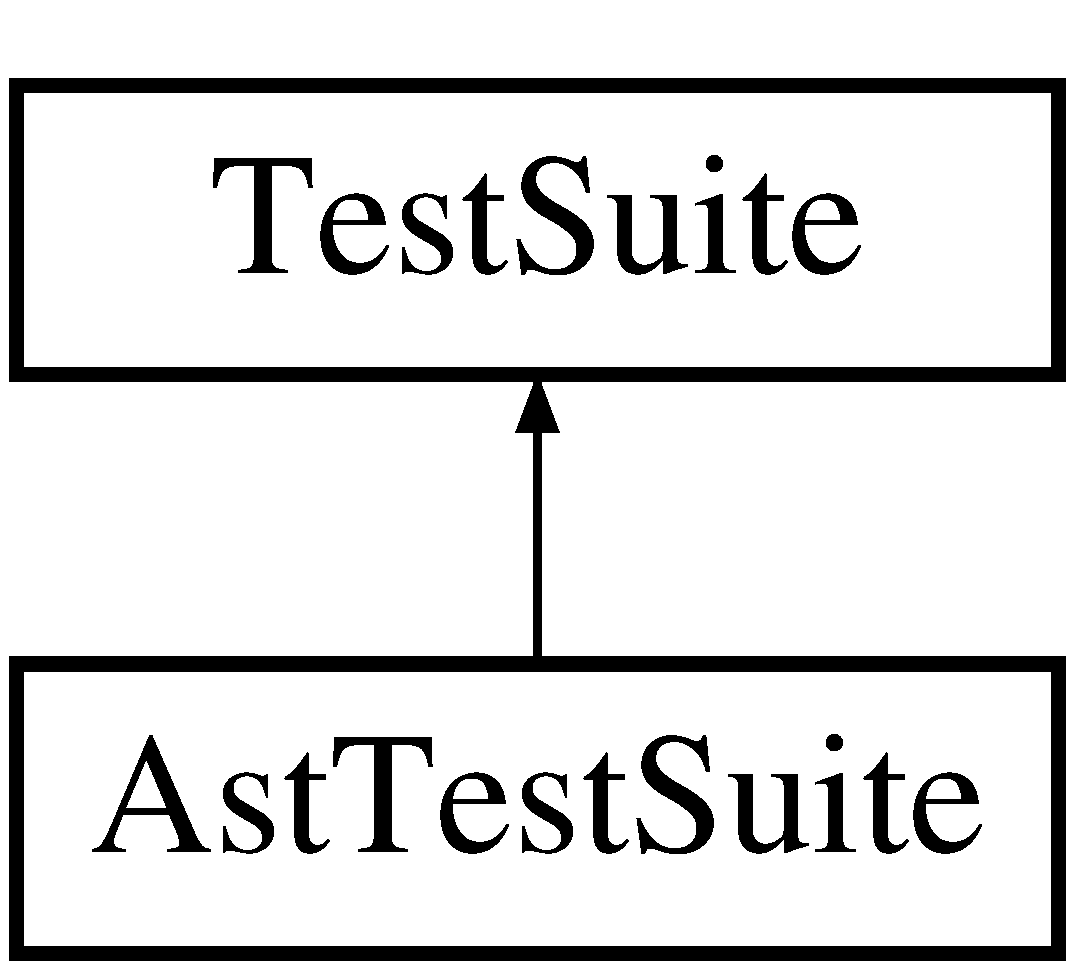
\includegraphics[height=2.000000cm]{classAstTestSuite}
\end{center}
\end{figure}
\subsection*{Public Member Functions}
\begin{DoxyCompactItemize}
\item 
\hypertarget{classAstTestSuite_a2f0462e7a965acda10e09e70432cab40}{char $\ast$$\ast$ {\bfseries make\-Args} (const char $\ast$a0, const char $\ast$a1)}\label{classAstTestSuite_a2f0462e7a965acda10e09e70432cab40}

\item 
\hypertarget{classAstTestSuite_ab935b3c95647b24b5f250b7e3332a313}{void {\bfseries write\-File} (const string text, const string filename)}\label{classAstTestSuite_ab935b3c95647b24b5f250b7e3332a313}

\item 
\hypertarget{classAstTestSuite_afb1462e2494b011f0e5077a567e0ba3d}{char $\ast$ {\bfseries read\-File} (const char $\ast$fn)}\label{classAstTestSuite_afb1462e2494b011f0e5077a567e0ba3d}

\item 
\hypertarget{classAstTestSuite_a1fb6dcbf82548632381eb89079b456aa}{void {\bfseries unparse\-\_\-tests} (string file)}\label{classAstTestSuite_a1fb6dcbf82548632381eb89079b456aa}

\item 
\hypertarget{classAstTestSuite_ade48304a65cbc7449bd22ec9097b6a8c}{void {\bfseries test\-\_\-sample\-\_\-1} (void)}\label{classAstTestSuite_ade48304a65cbc7449bd22ec9097b6a8c}

\item 
\hypertarget{classAstTestSuite_af764267aa9a94610fd5307ae81107312}{void {\bfseries test\-\_\-sample\-\_\-2} (void)}\label{classAstTestSuite_af764267aa9a94610fd5307ae81107312}

\item 
\hypertarget{classAstTestSuite_a956750fe55d2eb218eb75bd7dc75bc34}{void {\bfseries test\-\_\-sample\-\_\-3} (void)}\label{classAstTestSuite_a956750fe55d2eb218eb75bd7dc75bc34}

\item 
\hypertarget{classAstTestSuite_a665836b3d23c82eda3233a3c5d2f0ba4}{void {\bfseries test\-\_\-sample\-\_\-4} (void)}\label{classAstTestSuite_a665836b3d23c82eda3233a3c5d2f0ba4}

\item 
\hypertarget{classAstTestSuite_a9cceb7f0e5a6714d539f25db38424851}{void {\bfseries test\-\_\-sample\-\_\-5} (void)}\label{classAstTestSuite_a9cceb7f0e5a6714d539f25db38424851}

\item 
\hypertarget{classAstTestSuite_adbc7de61740aaf9ebf9b7e25f024f318}{void {\bfseries test\-\_\-mysample} (void)}\label{classAstTestSuite_adbc7de61740aaf9ebf9b7e25f024f318}

\item 
\hypertarget{classAstTestSuite_ade9231acfe5f8c8f02e00e54749cf99b}{void {\bfseries test\-\_\-forest\-\_\-loss} (void)}\label{classAstTestSuite_ade9231acfe5f8c8f02e00e54749cf99b}

\end{DoxyCompactItemize}
\subsection*{Public Attributes}
\begin{DoxyCompactItemize}
\item 
\hypertarget{classAstTestSuite_a148a26ab78abac732d857d7095f6dea5}{\hyperlink{classParser}{Parser} {\bfseries p}}\label{classAstTestSuite_a148a26ab78abac732d857d7095f6dea5}

\item 
\hypertarget{classAstTestSuite_ab27964f1743a2889538ca27e644eb1aa}{\hyperlink{classParseResult}{Parse\-Result} {\bfseries pr}}\label{classAstTestSuite_ab27964f1743a2889538ca27e644eb1aa}

\end{DoxyCompactItemize}


The documentation for this class was generated from the following file\-:\begin{DoxyCompactItemize}
\item 
ast\-\_\-tests.\-h\end{DoxyCompactItemize}

\hypertarget{structbestMatchRegex}{\section{best\-Match\-Regex Struct Reference}
\label{structbestMatchRegex}\index{best\-Match\-Regex@{best\-Match\-Regex}}
}
\subsection*{Public Attributes}
\begin{DoxyCompactItemize}
\item 
\hypertarget{structbestMatchRegex_a09f359d998398cf65e7d31a080eb2c01}{int {\bfseries num\-Matched}}\label{structbestMatchRegex_a09f359d998398cf65e7d31a080eb2c01}

\item 
\hypertarget{structbestMatchRegex_afef2c52de6332efd60cae71553bd9b0a}{token\-Type {\bfseries terminal}}\label{structbestMatchRegex_afef2c52de6332efd60cae71553bd9b0a}

\end{DoxyCompactItemize}


The documentation for this struct was generated from the following file\-:\begin{DoxyCompactItemize}
\item 
scanner.\-h\end{DoxyCompactItemize}

\hypertarget{classCharConstToken}{\section{Char\-Const\-Token Class Reference}
\label{classCharConstToken}\index{Char\-Const\-Token@{Char\-Const\-Token}}
}
Inheritance diagram for Char\-Const\-Token\-:\begin{figure}[H]
\begin{center}
\leavevmode
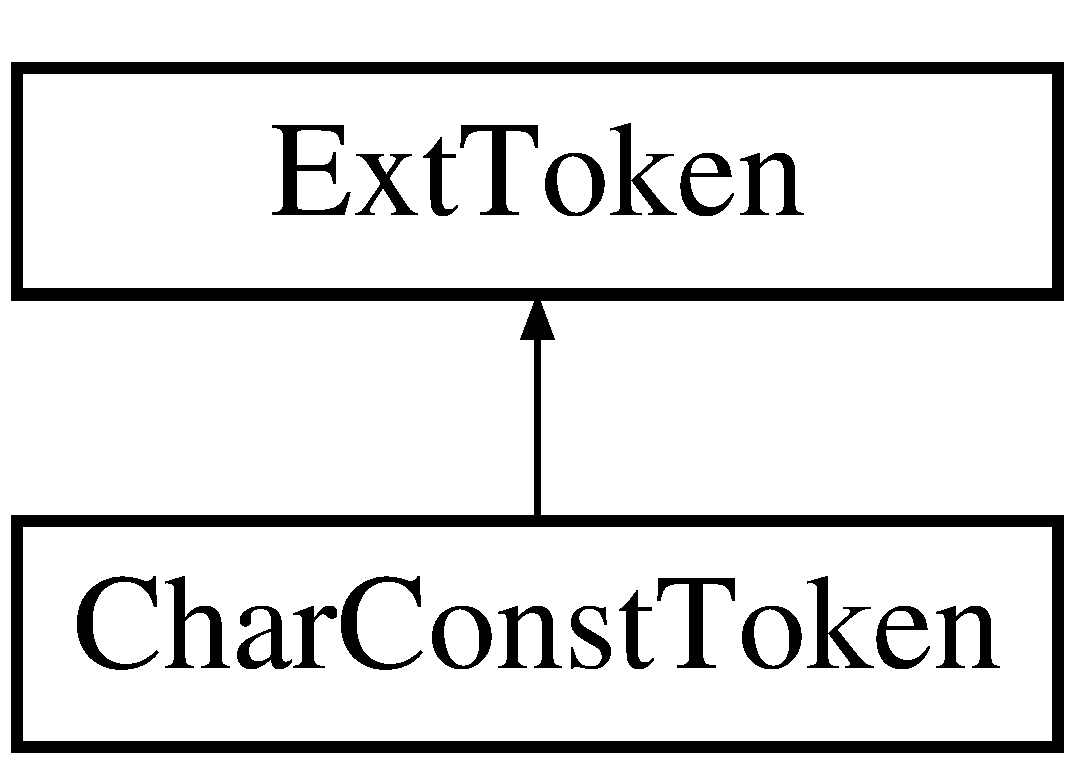
\includegraphics[height=2.000000cm]{classCharConstToken}
\end{center}
\end{figure}
\subsection*{Public Member Functions}
\begin{DoxyCompactItemize}
\item 
\hypertarget{classCharConstToken_a9dcb8d0d26c4f9c66570357641933c51}{{\bfseries Char\-Const\-Token} (\hyperlink{classParser}{Parser} $\ast$p, \hyperlink{classToken}{Token} $\ast$t)}\label{classCharConstToken_a9dcb8d0d26c4f9c66570357641933c51}

\item 
\hypertarget{classCharConstToken_a33032d6b35ef2b6ebc4db770b374ad5b}{\hyperlink{classParseResult}{Parse\-Result} {\bfseries nud} ()}\label{classCharConstToken_a33032d6b35ef2b6ebc4db770b374ad5b}

\item 
\hypertarget{classCharConstToken_addf2603d51bc2be908137f06737d8b30}{std\-::string {\bfseries description} ()}\label{classCharConstToken_addf2603d51bc2be908137f06737d8b30}

\end{DoxyCompactItemize}
\subsection*{Additional Inherited Members}


The documentation for this class was generated from the following file\-:\begin{DoxyCompactItemize}
\item 
ext\-Token.\-h\end{DoxyCompactItemize}

\hypertarget{classDashToken}{\section{Dash\-Token Class Reference}
\label{classDashToken}\index{Dash\-Token@{Dash\-Token}}
}
Inheritance diagram for Dash\-Token\-:\begin{figure}[H]
\begin{center}
\leavevmode
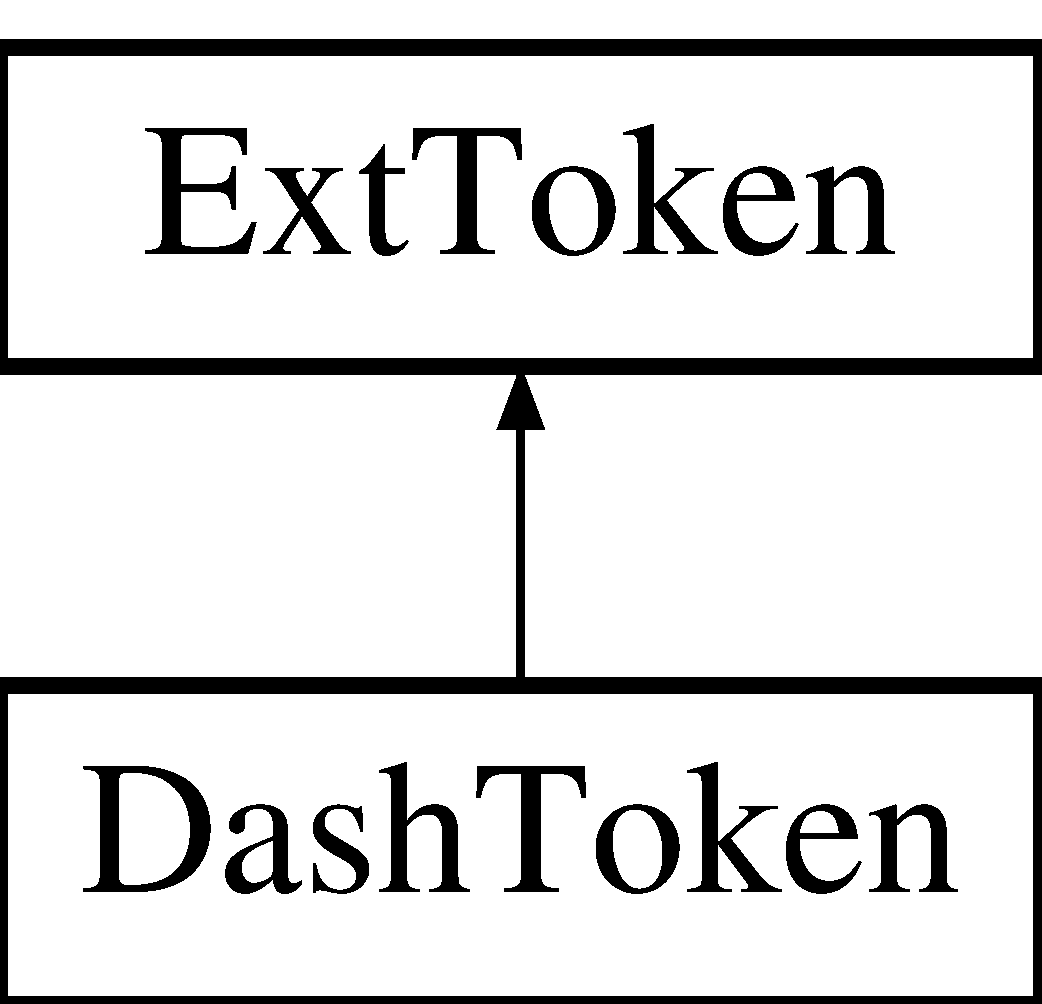
\includegraphics[height=2.000000cm]{classDashToken}
\end{center}
\end{figure}
\subsection*{Public Member Functions}
\begin{DoxyCompactItemize}
\item 
\hypertarget{classDashToken_a9570d66563405c728e679b63a44e53e2}{{\bfseries Dash\-Token} (\hyperlink{classParser}{Parser} $\ast$p, \hyperlink{classToken}{Token} $\ast$t)}\label{classDashToken_a9570d66563405c728e679b63a44e53e2}

\item 
\hypertarget{classDashToken_a703ca6afcd05ac4688c66b82e177bdbc}{\hyperlink{classParseResult}{Parse\-Result} {\bfseries led} (\hyperlink{classParseResult}{Parse\-Result} left)}\label{classDashToken_a703ca6afcd05ac4688c66b82e177bdbc}

\item 
\hypertarget{classDashToken_a02d79abb30dcab20081edb8e969885d2}{std\-::string {\bfseries description} ()}\label{classDashToken_a02d79abb30dcab20081edb8e969885d2}

\item 
\hypertarget{classDashToken_a1cf877584a85c06e884a182744e92b39}{int {\bfseries lbp} ()}\label{classDashToken_a1cf877584a85c06e884a182744e92b39}

\end{DoxyCompactItemize}
\subsection*{Additional Inherited Members}


The documentation for this class was generated from the following file\-:\begin{DoxyCompactItemize}
\item 
ext\-Token.\-h\end{DoxyCompactItemize}

\hypertarget{classDecl}{\section{Decl Class Reference}
\label{classDecl}\index{Decl@{Decl}}
}
Inheritance diagram for Decl\-:\begin{figure}[H]
\begin{center}
\leavevmode
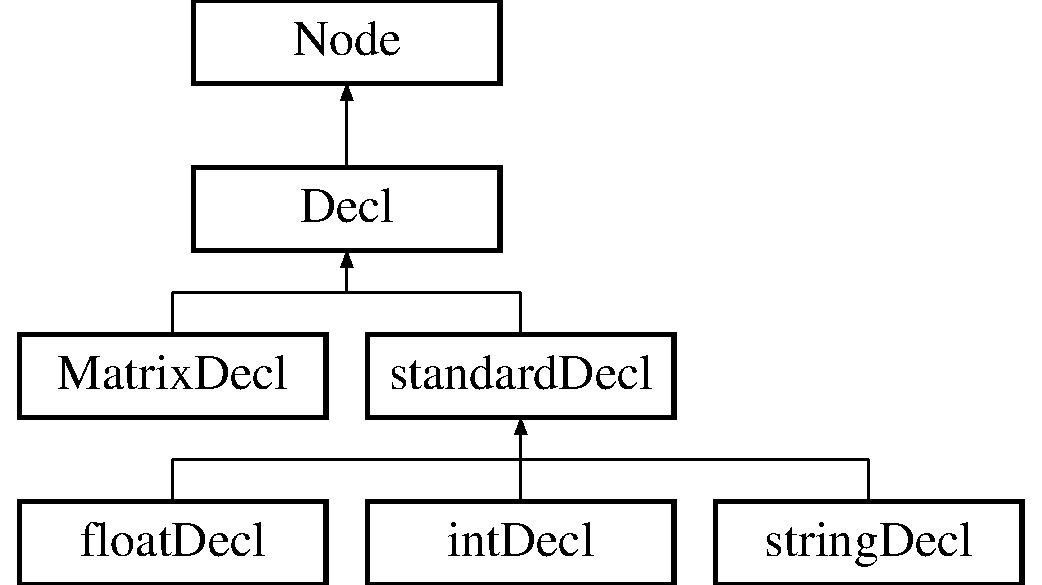
\includegraphics[height=4.000000cm]{classDecl}
\end{center}
\end{figure}
\subsection*{Additional Inherited Members}


The documentation for this class was generated from the following file\-:\begin{DoxyCompactItemize}
\item 
A\-S\-T.\-h\end{DoxyCompactItemize}

\hypertarget{classEndOfFileToken}{\section{End\-Of\-File\-Token Class Reference}
\label{classEndOfFileToken}\index{End\-Of\-File\-Token@{End\-Of\-File\-Token}}
}
Inheritance diagram for End\-Of\-File\-Token\-:\begin{figure}[H]
\begin{center}
\leavevmode
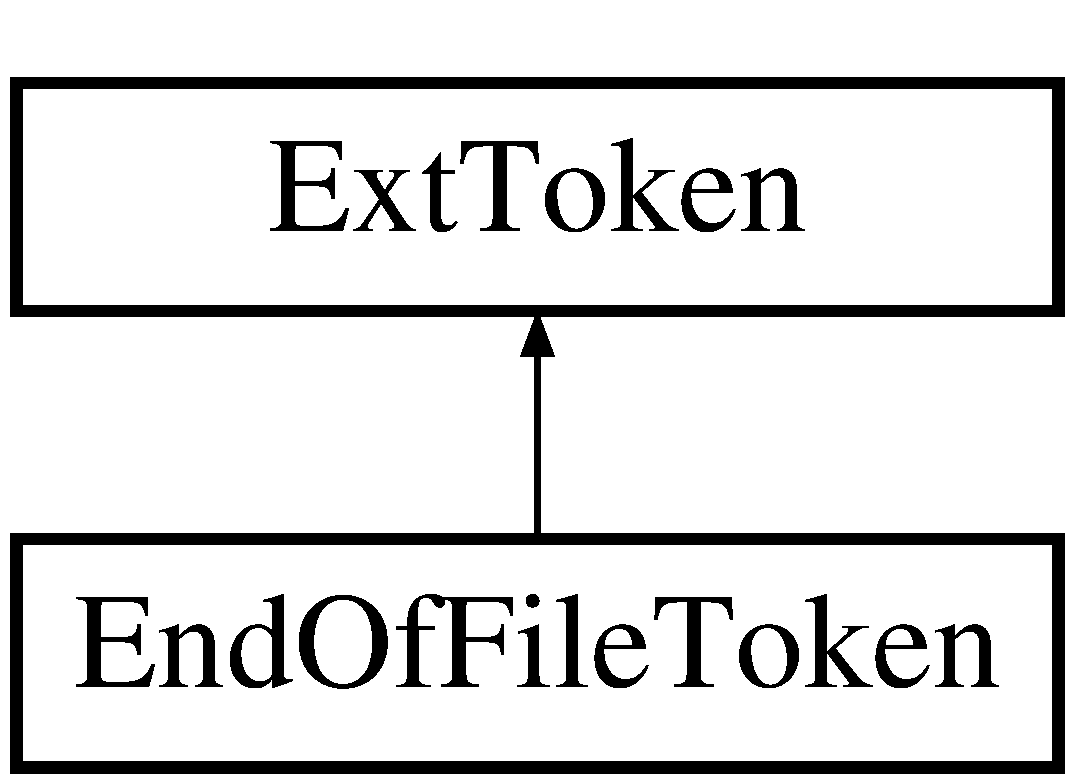
\includegraphics[height=2.000000cm]{classEndOfFileToken}
\end{center}
\end{figure}
\subsection*{Public Member Functions}
\begin{DoxyCompactItemize}
\item 
\hypertarget{classEndOfFileToken_a5c093bc13648a4f4df525ea4242e59d9}{{\bfseries End\-Of\-File\-Token} (\hyperlink{classParser}{Parser} $\ast$p, \hyperlink{classToken}{Token} $\ast$t)}\label{classEndOfFileToken_a5c093bc13648a4f4df525ea4242e59d9}

\item 
\hypertarget{classEndOfFileToken_a918312b101ca8cc7fb5ba4e56bc12b58}{std\-::string {\bfseries description} ()}\label{classEndOfFileToken_a918312b101ca8cc7fb5ba4e56bc12b58}

\end{DoxyCompactItemize}
\subsection*{Additional Inherited Members}


The documentation for this class was generated from the following file\-:\begin{DoxyCompactItemize}
\item 
ext\-Token.\-h\end{DoxyCompactItemize}

\hypertarget{classExtToken}{\section{Ext\-Token Class Reference}
\label{classExtToken}\index{Ext\-Token@{Ext\-Token}}
}
Inheritance diagram for Ext\-Token\-:\begin{figure}[H]
\begin{center}
\leavevmode
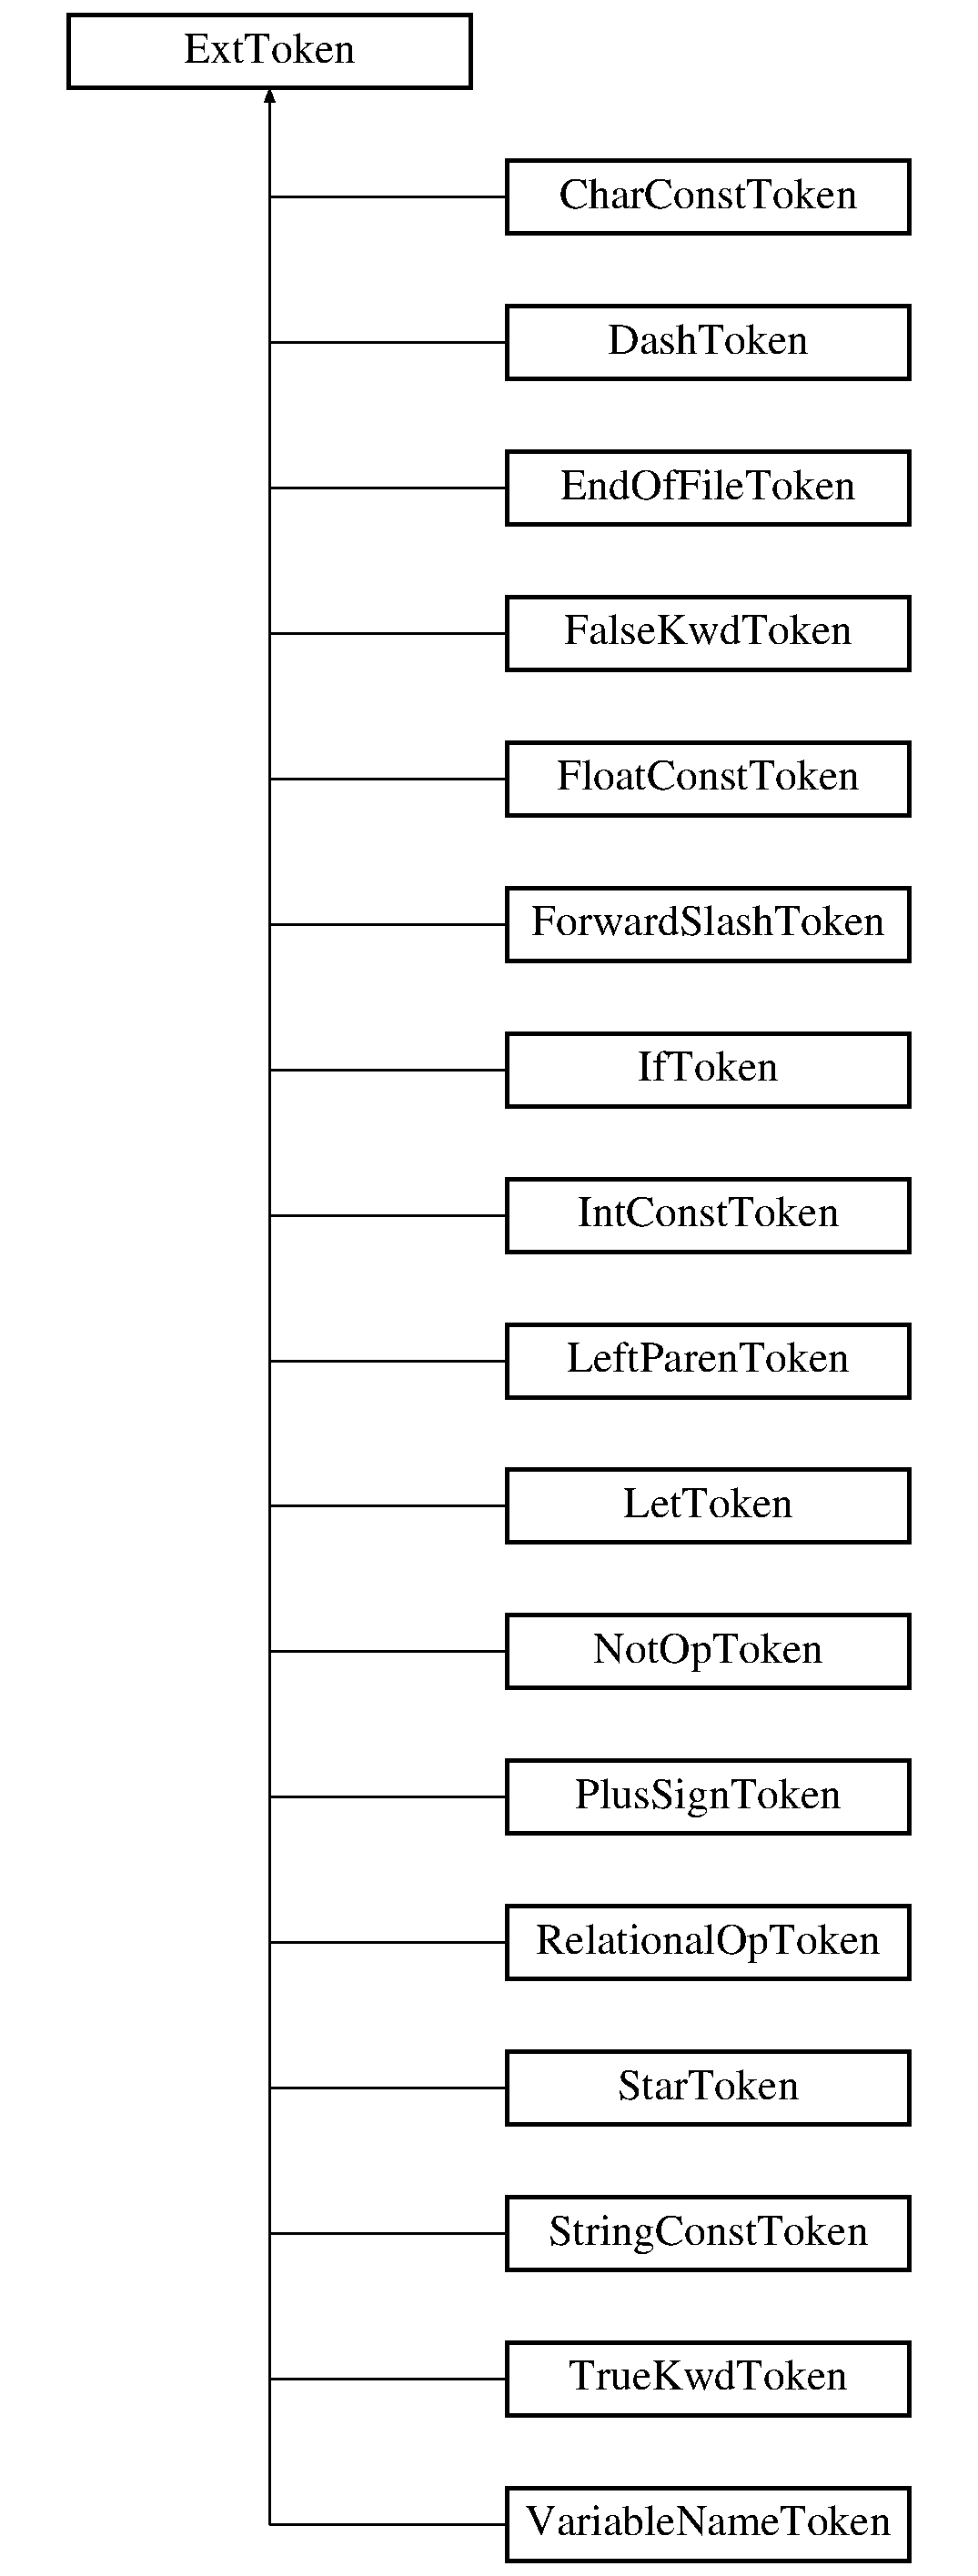
\includegraphics[height=12.000000cm]{classExtToken}
\end{center}
\end{figure}
\subsection*{Public Member Functions}
\begin{DoxyCompactItemize}
\item 
\hypertarget{classExtToken_a45a27528f391faf5679b7b30563ce846}{{\bfseries Ext\-Token} (\hyperlink{classParser}{Parser} $\ast$p, \hyperlink{classToken}{Token} $\ast$t)}\label{classExtToken_a45a27528f391faf5679b7b30563ce846}

\item 
\hypertarget{classExtToken_afa8972152abec42cd52b6f6f70a9a179}{{\bfseries Ext\-Token} (\hyperlink{classParser}{Parser} $\ast$p, \hyperlink{classToken}{Token} $\ast$t, std\-::string d)}\label{classExtToken_afa8972152abec42cd52b6f6f70a9a179}

\item 
\hypertarget{classExtToken_a5c21a5ffe91f212085259126652ab77c}{virtual \hyperlink{classParseResult}{Parse\-Result} {\bfseries nud} ()}\label{classExtToken_a5c21a5ffe91f212085259126652ab77c}

\item 
\hypertarget{classExtToken_afb2c9b0040e198d1d8aa2e041c5a7211}{virtual \hyperlink{classParseResult}{Parse\-Result} {\bfseries led} (\hyperlink{classParseResult}{Parse\-Result} left)}\label{classExtToken_afb2c9b0040e198d1d8aa2e041c5a7211}

\item 
\hypertarget{classExtToken_a6c0d61faa058b71147dd54bacee1db94}{virtual int {\bfseries lbp} ()}\label{classExtToken_a6c0d61faa058b71147dd54bacee1db94}

\item 
\hypertarget{classExtToken_a4ab6e72ac23235650b1756f794172ebb}{virtual std\-::string {\bfseries description} ()}\label{classExtToken_a4ab6e72ac23235650b1756f794172ebb}

\end{DoxyCompactItemize}
\subsection*{Public Attributes}
\begin{DoxyCompactItemize}
\item 
\hypertarget{classExtToken_a5af1643a542ef7ee8ca0f82706383ae3}{std\-::string {\bfseries lexeme}}\label{classExtToken_a5af1643a542ef7ee8ca0f82706383ae3}

\item 
\hypertarget{classExtToken_abbdaef42b65403cdc0247839ef95c875}{token\-Type {\bfseries terminal}}\label{classExtToken_abbdaef42b65403cdc0247839ef95c875}

\item 
\hypertarget{classExtToken_aa02995a897183b2a6ef758e541534e46}{\hyperlink{classExtToken}{Ext\-Token} $\ast$ {\bfseries next}}\label{classExtToken_aa02995a897183b2a6ef758e541534e46}

\item 
\hypertarget{classExtToken_af70d22156d5f8e855a8b0d92a82706ba}{\hyperlink{classParser}{Parser} $\ast$ {\bfseries parser}}\label{classExtToken_af70d22156d5f8e855a8b0d92a82706ba}

\end{DoxyCompactItemize}


The documentation for this class was generated from the following file\-:\begin{DoxyCompactItemize}
\item 
ext\-Token.\-h\end{DoxyCompactItemize}

\hypertarget{classFalseKwdToken}{\section{False\-Kwd\-Token Class Reference}
\label{classFalseKwdToken}\index{False\-Kwd\-Token@{False\-Kwd\-Token}}
}
Inheritance diagram for False\-Kwd\-Token\-:\begin{figure}[H]
\begin{center}
\leavevmode
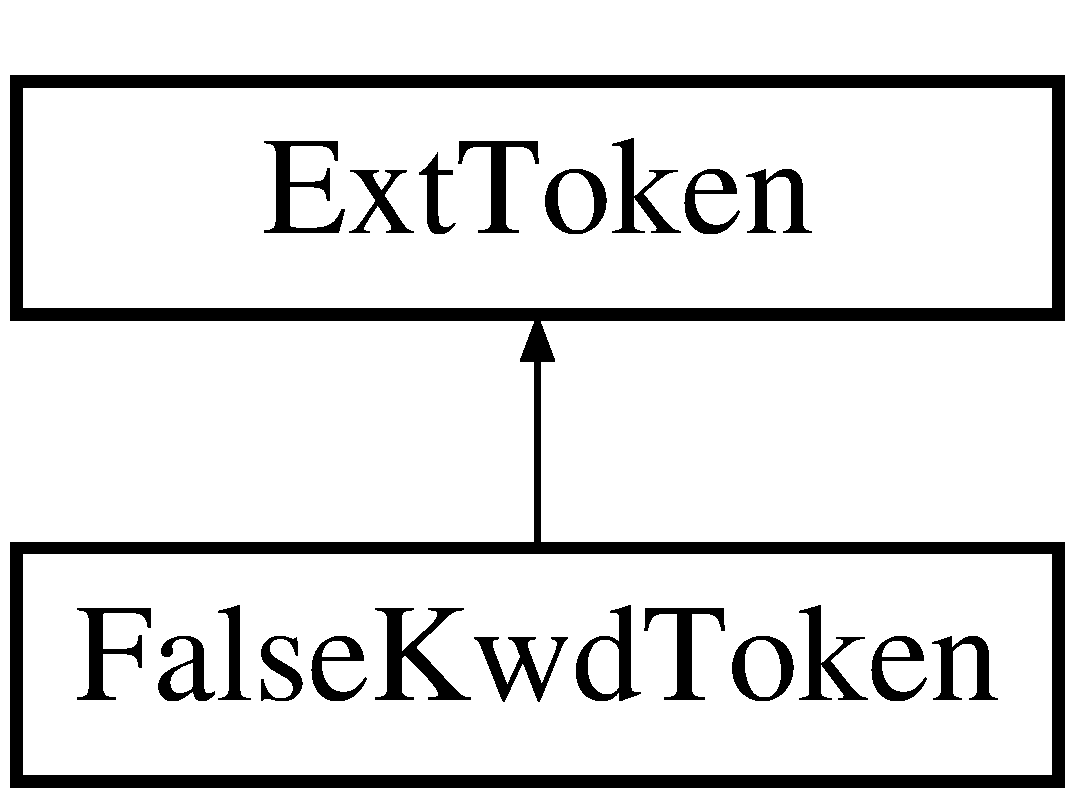
\includegraphics[height=2.000000cm]{classFalseKwdToken}
\end{center}
\end{figure}
\subsection*{Public Member Functions}
\begin{DoxyCompactItemize}
\item 
\hypertarget{classFalseKwdToken_add6402d29fd7b22253a0dc73370597e4}{{\bfseries False\-Kwd\-Token} (\hyperlink{classParser}{Parser} $\ast$p, \hyperlink{classToken}{Token} $\ast$t)}\label{classFalseKwdToken_add6402d29fd7b22253a0dc73370597e4}

\item 
\hypertarget{classFalseKwdToken_adc06b0433535d552c1e7f8076d756fb3}{\hyperlink{classParseResult}{Parse\-Result} {\bfseries nud} ()}\label{classFalseKwdToken_adc06b0433535d552c1e7f8076d756fb3}

\item 
\hypertarget{classFalseKwdToken_a8351fad7090214687138e113b5a581f1}{std\-::string {\bfseries description} ()}\label{classFalseKwdToken_a8351fad7090214687138e113b5a581f1}

\end{DoxyCompactItemize}
\subsection*{Additional Inherited Members}


The documentation for this class was generated from the following file\-:\begin{DoxyCompactItemize}
\item 
ext\-Token.\-h\end{DoxyCompactItemize}

\hypertarget{classFloatConstToken}{\section{Float\-Const\-Token Class Reference}
\label{classFloatConstToken}\index{Float\-Const\-Token@{Float\-Const\-Token}}
}
Inheritance diagram for Float\-Const\-Token\-:\begin{figure}[H]
\begin{center}
\leavevmode
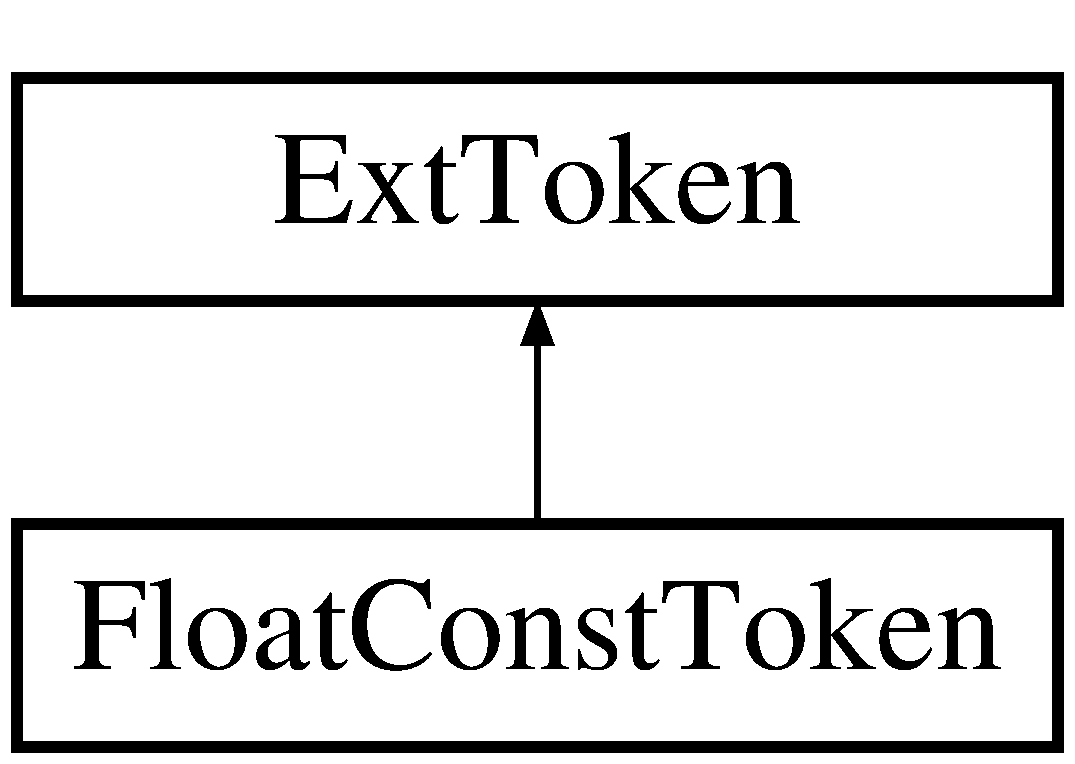
\includegraphics[height=2.000000cm]{classFloatConstToken}
\end{center}
\end{figure}
\subsection*{Public Member Functions}
\begin{DoxyCompactItemize}
\item 
\hypertarget{classFloatConstToken_aecee1d0e4e8a9410701c68c30858a4db}{{\bfseries Float\-Const\-Token} (\hyperlink{classParser}{Parser} $\ast$p, \hyperlink{classToken}{Token} $\ast$t)}\label{classFloatConstToken_aecee1d0e4e8a9410701c68c30858a4db}

\item 
\hypertarget{classFloatConstToken_a991e92ae34d0b01a3b1dd08ed01b8e6e}{\hyperlink{classParseResult}{Parse\-Result} {\bfseries nud} ()}\label{classFloatConstToken_a991e92ae34d0b01a3b1dd08ed01b8e6e}

\item 
\hypertarget{classFloatConstToken_a529b6d3ad479b0f6b940a82ba48b98c0}{std\-::string {\bfseries description} ()}\label{classFloatConstToken_a529b6d3ad479b0f6b940a82ba48b98c0}

\end{DoxyCompactItemize}
\subsection*{Additional Inherited Members}


The documentation for this class was generated from the following file\-:\begin{DoxyCompactItemize}
\item 
ext\-Token.\-h\end{DoxyCompactItemize}

\hypertarget{classfloatDecl}{\section{float\-Decl Class Reference}
\label{classfloatDecl}\index{float\-Decl@{float\-Decl}}
}
Inheritance diagram for float\-Decl\-:\begin{figure}[H]
\begin{center}
\leavevmode
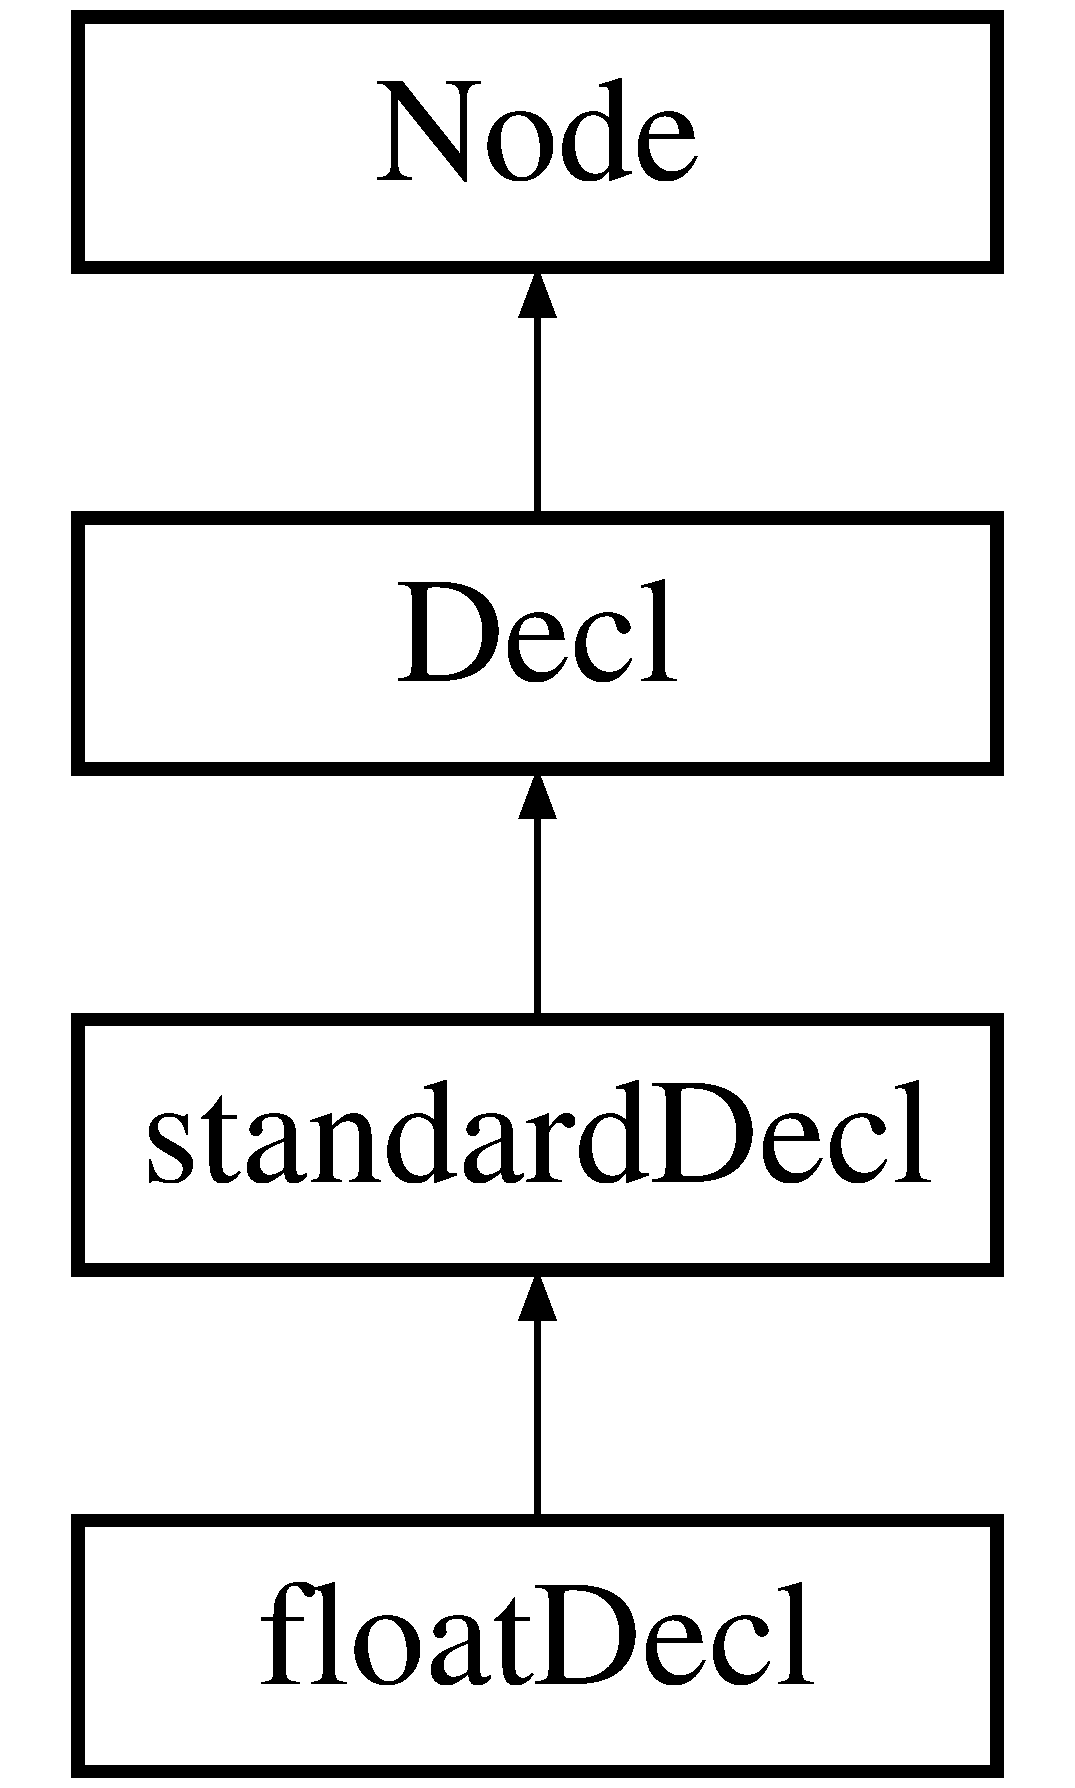
\includegraphics[height=4.000000cm]{classfloatDecl}
\end{center}
\end{figure}
\subsection*{Additional Inherited Members}


The documentation for this class was generated from the following file\-:\begin{DoxyCompactItemize}
\item 
A\-S\-T.\-h\end{DoxyCompactItemize}

\hypertarget{classForwardSlashToken}{\section{Forward\-Slash\-Token Class Reference}
\label{classForwardSlashToken}\index{Forward\-Slash\-Token@{Forward\-Slash\-Token}}
}
Inheritance diagram for Forward\-Slash\-Token\-:\begin{figure}[H]
\begin{center}
\leavevmode
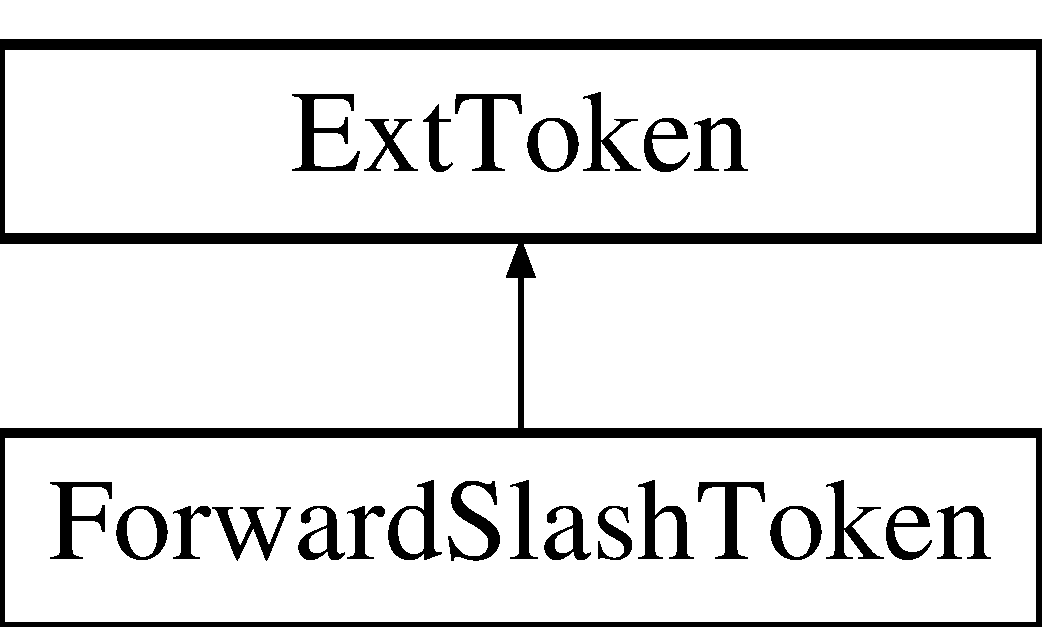
\includegraphics[height=2.000000cm]{classForwardSlashToken}
\end{center}
\end{figure}
\subsection*{Public Member Functions}
\begin{DoxyCompactItemize}
\item 
\hypertarget{classForwardSlashToken_ae818840269cd15f6f6b00929fb4eb979}{{\bfseries Forward\-Slash\-Token} (\hyperlink{classParser}{Parser} $\ast$p, \hyperlink{classToken}{Token} $\ast$t)}\label{classForwardSlashToken_ae818840269cd15f6f6b00929fb4eb979}

\item 
\hypertarget{classForwardSlashToken_ac2dda7b791ab555e4323f17baaf323e1}{\hyperlink{classParseResult}{Parse\-Result} {\bfseries led} (\hyperlink{classParseResult}{Parse\-Result} left)}\label{classForwardSlashToken_ac2dda7b791ab555e4323f17baaf323e1}

\item 
\hypertarget{classForwardSlashToken_ac27b1ab175ec08c468bd0d4c41636a5c}{std\-::string {\bfseries description} ()}\label{classForwardSlashToken_ac27b1ab175ec08c468bd0d4c41636a5c}

\item 
\hypertarget{classForwardSlashToken_ad65829044355922a291dfbfd3052b183}{int {\bfseries lbp} ()}\label{classForwardSlashToken_ad65829044355922a291dfbfd3052b183}

\end{DoxyCompactItemize}
\subsection*{Additional Inherited Members}


The documentation for this class was generated from the following file\-:\begin{DoxyCompactItemize}
\item 
ext\-Token.\-h\end{DoxyCompactItemize}

\hypertarget{classIfToken}{\section{If\-Token Class Reference}
\label{classIfToken}\index{If\-Token@{If\-Token}}
}
Inheritance diagram for If\-Token\-:\begin{figure}[H]
\begin{center}
\leavevmode
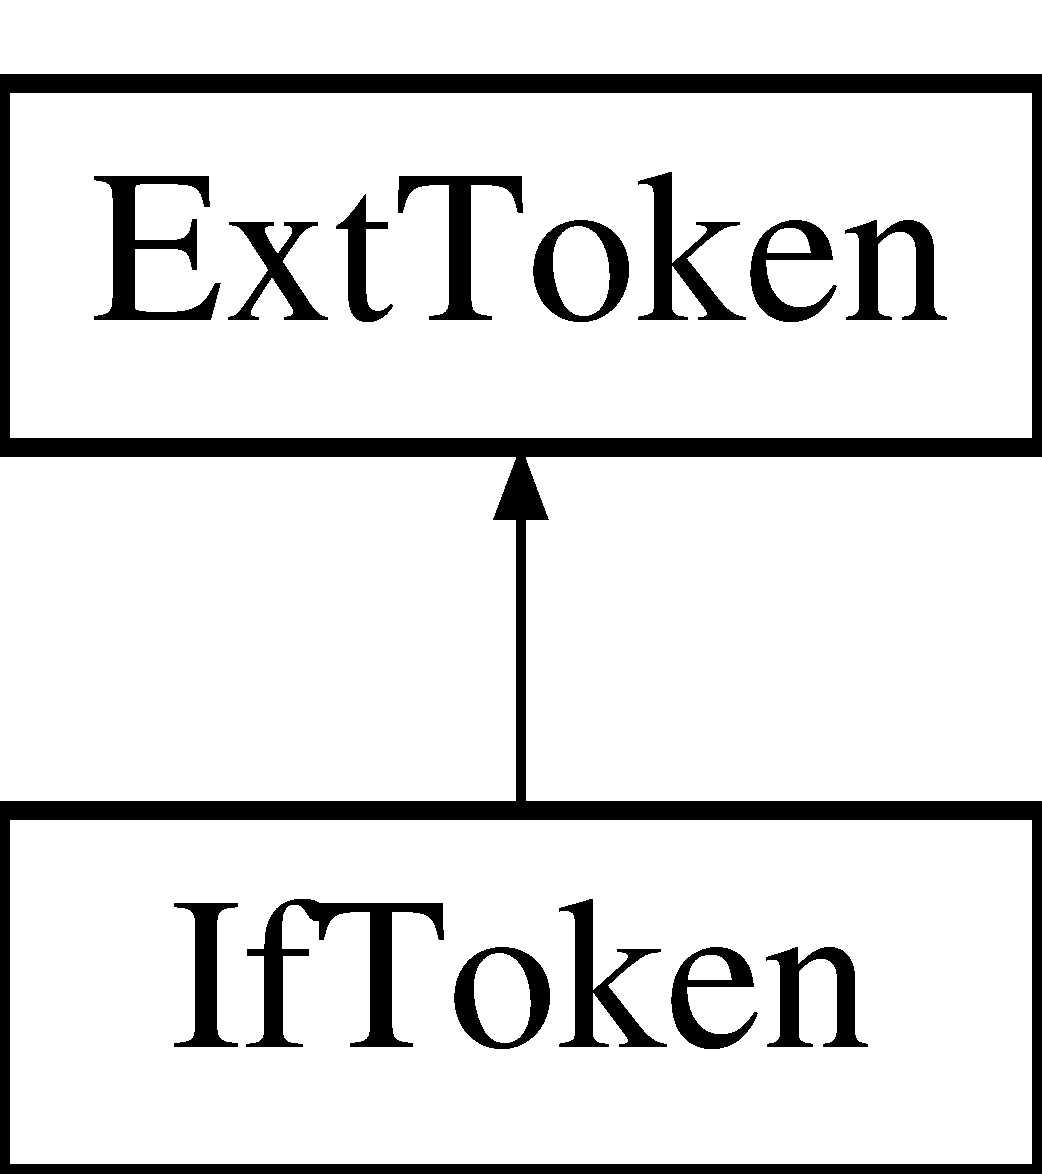
\includegraphics[height=2.000000cm]{classIfToken}
\end{center}
\end{figure}
\subsection*{Public Member Functions}
\begin{DoxyCompactItemize}
\item 
\hypertarget{classIfToken_a607028595b06b8a950000ba3e82329db}{{\bfseries If\-Token} (\hyperlink{classParser}{Parser} $\ast$p, \hyperlink{classToken}{Token} $\ast$t)}\label{classIfToken_a607028595b06b8a950000ba3e82329db}

\item 
\hypertarget{classIfToken_add06bd79ce755fd5503f78e507109e52}{\hyperlink{classParseResult}{Parse\-Result} {\bfseries nud} ()}\label{classIfToken_add06bd79ce755fd5503f78e507109e52}

\item 
\hypertarget{classIfToken_aad226162c5649920c13c2a9e9e7a3617}{std\-::string {\bfseries description} ()}\label{classIfToken_aad226162c5649920c13c2a9e9e7a3617}

\item 
\hypertarget{classIfToken_abfd39ff4c4818d382bf0b97fd097c478}{int {\bfseries lbp} ()}\label{classIfToken_abfd39ff4c4818d382bf0b97fd097c478}

\end{DoxyCompactItemize}
\subsection*{Additional Inherited Members}


The documentation for this class was generated from the following file\-:\begin{DoxyCompactItemize}
\item 
ext\-Token.\-h\end{DoxyCompactItemize}

\hypertarget{classIntConstToken}{\section{Int\-Const\-Token Class Reference}
\label{classIntConstToken}\index{Int\-Const\-Token@{Int\-Const\-Token}}
}
Inheritance diagram for Int\-Const\-Token\-:\begin{figure}[H]
\begin{center}
\leavevmode
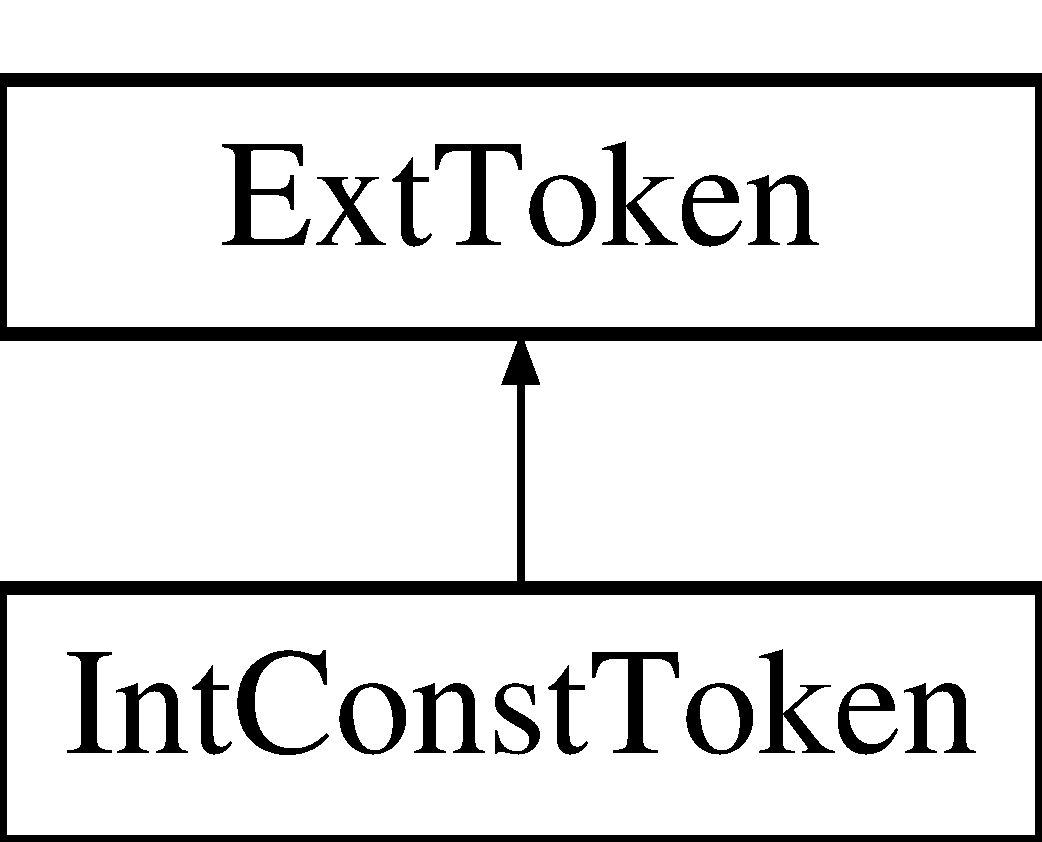
\includegraphics[height=2.000000cm]{classIntConstToken}
\end{center}
\end{figure}
\subsection*{Public Member Functions}
\begin{DoxyCompactItemize}
\item 
\hypertarget{classIntConstToken_a14c6bf0af5a915969b4fef1758067af3}{{\bfseries Int\-Const\-Token} (\hyperlink{classParser}{Parser} $\ast$p, \hyperlink{classToken}{Token} $\ast$t)}\label{classIntConstToken_a14c6bf0af5a915969b4fef1758067af3}

\item 
\hypertarget{classIntConstToken_ae1f720d6006c47e145cae7879d09c708}{\hyperlink{classParseResult}{Parse\-Result} {\bfseries nud} ()}\label{classIntConstToken_ae1f720d6006c47e145cae7879d09c708}

\item 
\hypertarget{classIntConstToken_a98191508d849878d40800e447a0f1892}{std\-::string {\bfseries description} ()}\label{classIntConstToken_a98191508d849878d40800e447a0f1892}

\end{DoxyCompactItemize}
\subsection*{Additional Inherited Members}


The documentation for this class was generated from the following file\-:\begin{DoxyCompactItemize}
\item 
ext\-Token.\-h\end{DoxyCompactItemize}

\hypertarget{classintDecl}{\section{int\-Decl Class Reference}
\label{classintDecl}\index{int\-Decl@{int\-Decl}}
}
Inheritance diagram for int\-Decl\-:\begin{figure}[H]
\begin{center}
\leavevmode
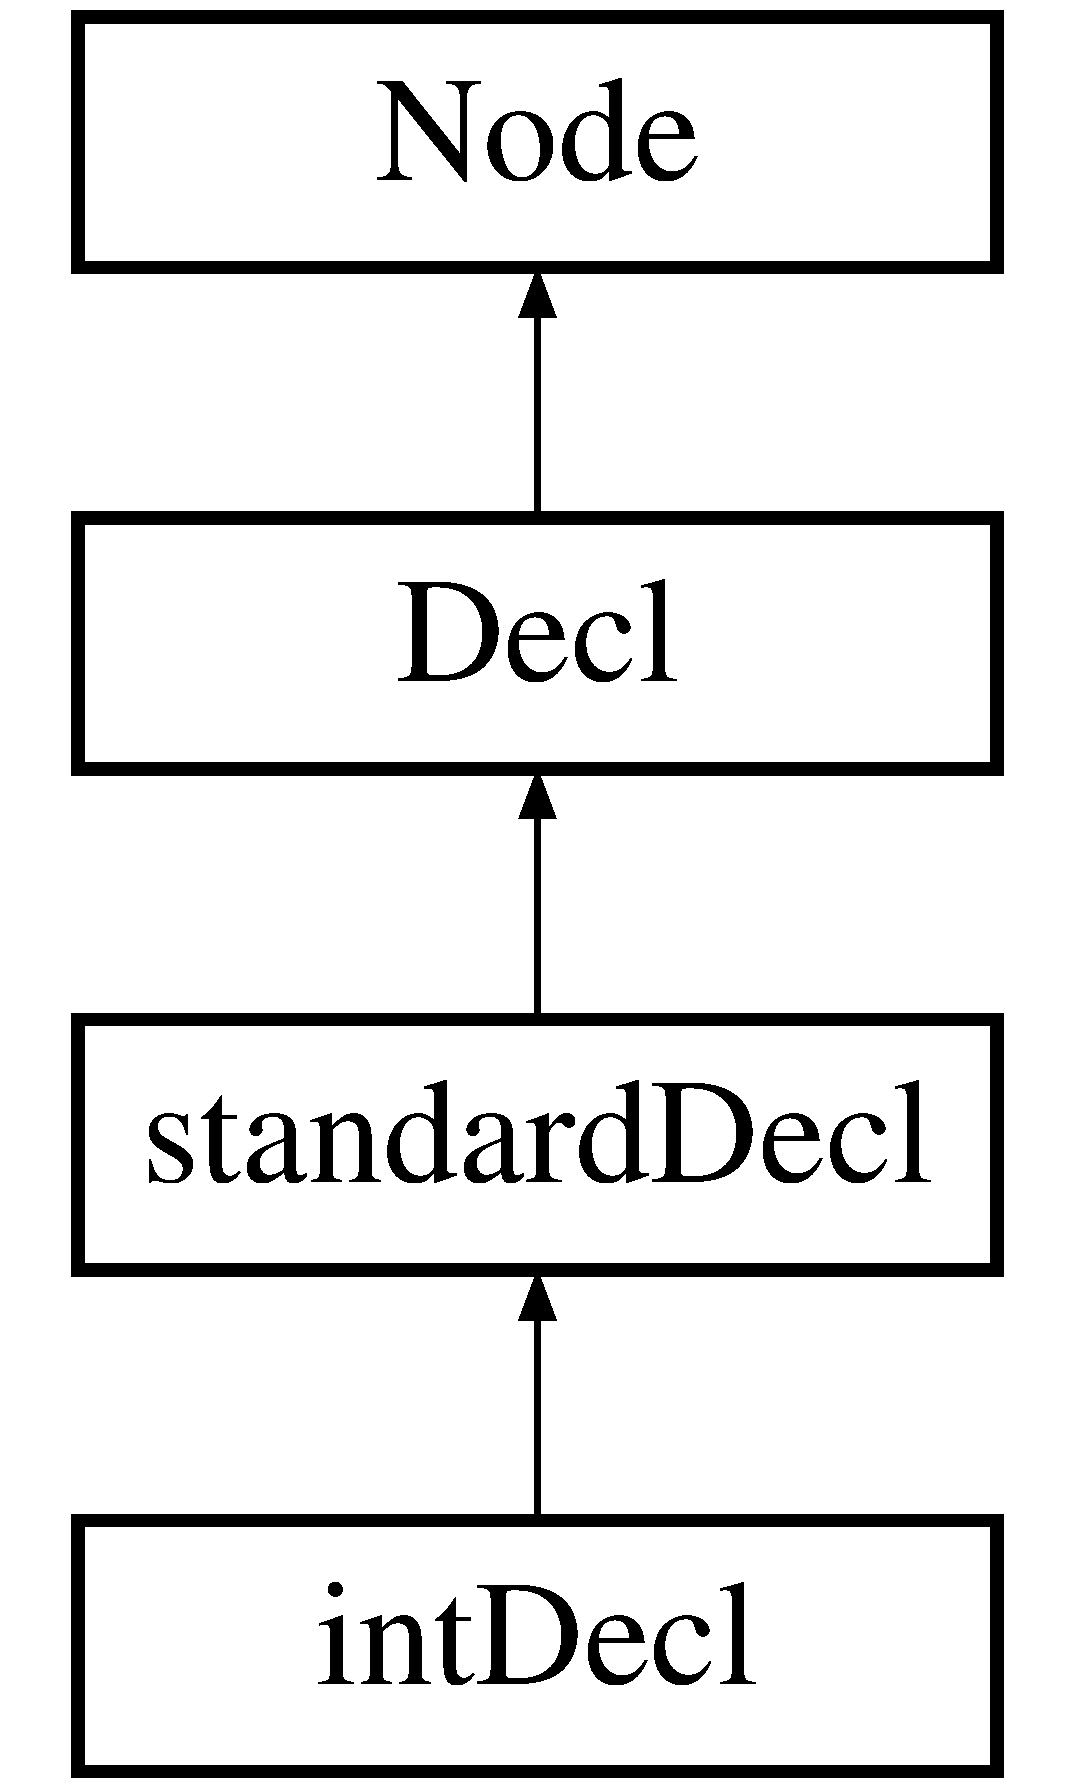
\includegraphics[height=4.000000cm]{classintDecl}
\end{center}
\end{figure}
\subsection*{Additional Inherited Members}


The documentation for this class was generated from the following file\-:\begin{DoxyCompactItemize}
\item 
A\-S\-T.\-h\end{DoxyCompactItemize}

\hypertarget{classLeftParenToken}{\section{Left\-Paren\-Token Class Reference}
\label{classLeftParenToken}\index{Left\-Paren\-Token@{Left\-Paren\-Token}}
}
Inheritance diagram for Left\-Paren\-Token\-:\begin{figure}[H]
\begin{center}
\leavevmode
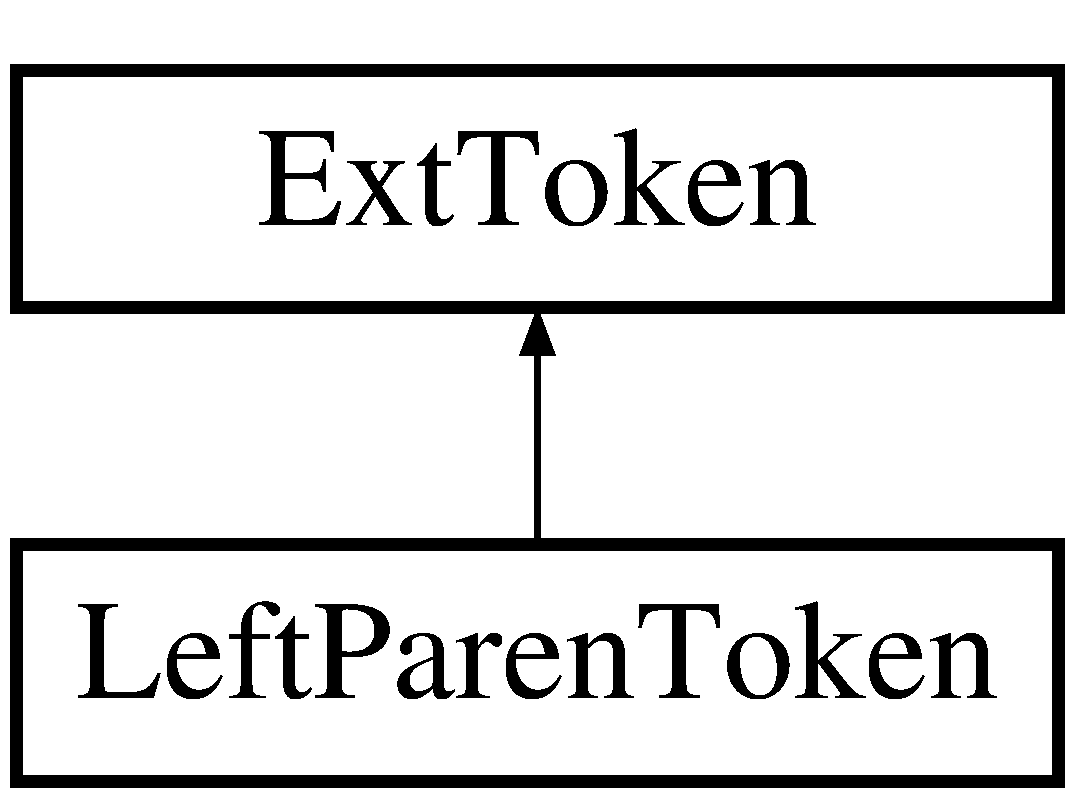
\includegraphics[height=2.000000cm]{classLeftParenToken}
\end{center}
\end{figure}
\subsection*{Public Member Functions}
\begin{DoxyCompactItemize}
\item 
\hypertarget{classLeftParenToken_aecdc6faf48a1a7192ec55712f0264cba}{{\bfseries Left\-Paren\-Token} (\hyperlink{classParser}{Parser} $\ast$p, \hyperlink{classToken}{Token} $\ast$t)}\label{classLeftParenToken_aecdc6faf48a1a7192ec55712f0264cba}

\item 
\hypertarget{classLeftParenToken_a3cb3ae9ab2647e5534c85529d314f08b}{\hyperlink{classParseResult}{Parse\-Result} {\bfseries nud} ()}\label{classLeftParenToken_a3cb3ae9ab2647e5534c85529d314f08b}

\item 
\hypertarget{classLeftParenToken_a2df35684bd2081c3bdfe2357946917bc}{std\-::string {\bfseries description} ()}\label{classLeftParenToken_a2df35684bd2081c3bdfe2357946917bc}

\item 
\hypertarget{classLeftParenToken_afa1b94645278f097bb097d3b24445d14}{int {\bfseries lbp} ()}\label{classLeftParenToken_afa1b94645278f097bb097d3b24445d14}

\end{DoxyCompactItemize}
\subsection*{Additional Inherited Members}


The documentation for this class was generated from the following file\-:\begin{DoxyCompactItemize}
\item 
ext\-Token.\-h\end{DoxyCompactItemize}

\hypertarget{classLetToken}{\section{Let\-Token Class Reference}
\label{classLetToken}\index{Let\-Token@{Let\-Token}}
}
Inheritance diagram for Let\-Token\-:\begin{figure}[H]
\begin{center}
\leavevmode
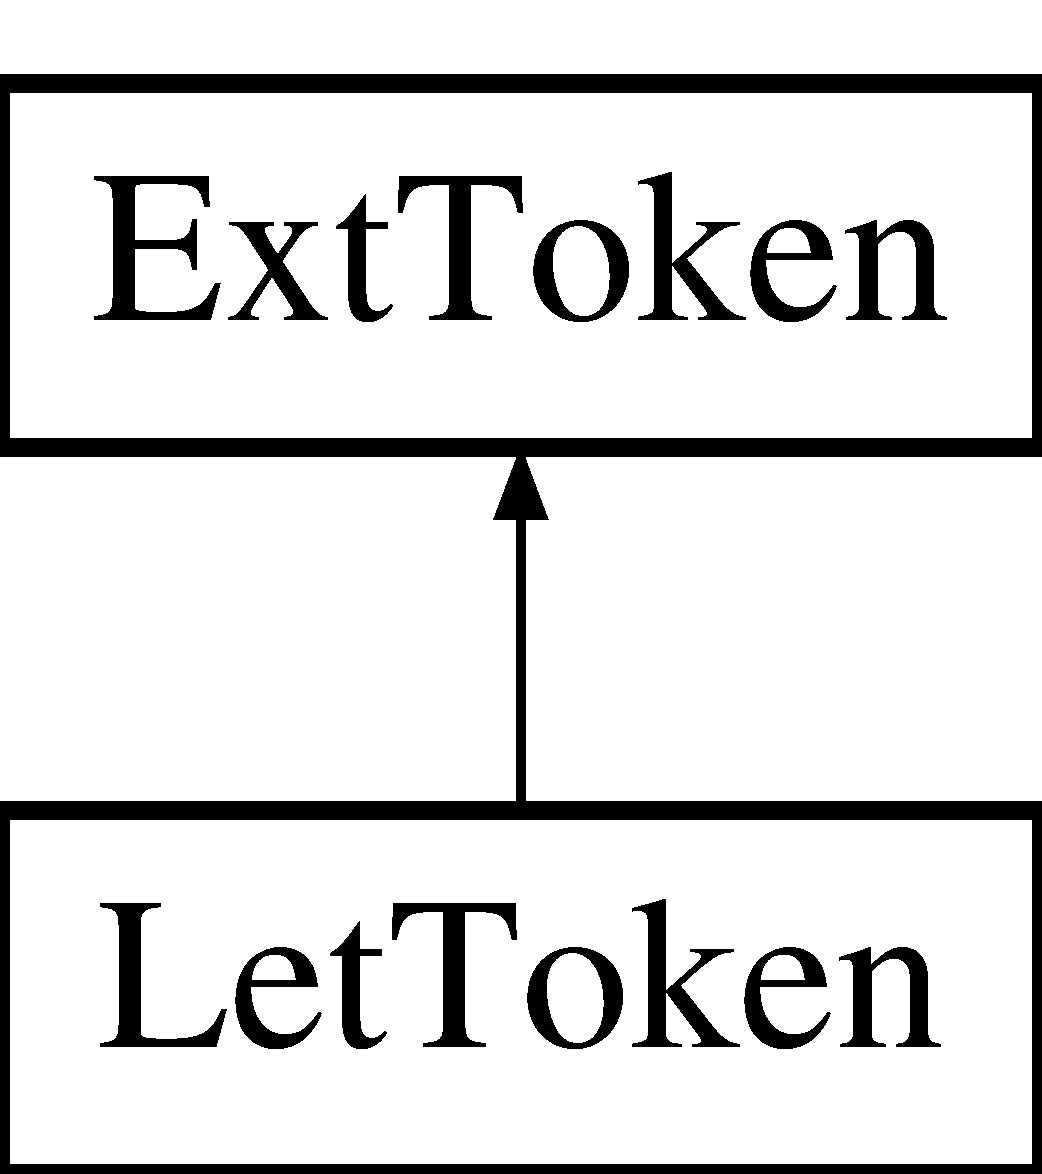
\includegraphics[height=2.000000cm]{classLetToken}
\end{center}
\end{figure}
\subsection*{Public Member Functions}
\begin{DoxyCompactItemize}
\item 
\hypertarget{classLetToken_a94651a82207e47cd2c1066a58cb1fe08}{{\bfseries Let\-Token} (\hyperlink{classParser}{Parser} $\ast$p, \hyperlink{classToken}{Token} $\ast$t)}\label{classLetToken_a94651a82207e47cd2c1066a58cb1fe08}

\item 
\hypertarget{classLetToken_a14df948cdf775bde8392bf58d53b91f3}{\hyperlink{classParseResult}{Parse\-Result} {\bfseries nud} ()}\label{classLetToken_a14df948cdf775bde8392bf58d53b91f3}

\item 
\hypertarget{classLetToken_a2c5ba0489774bf6468a26f4e19d7fab4}{std\-::string {\bfseries description} ()}\label{classLetToken_a2c5ba0489774bf6468a26f4e19d7fab4}

\item 
\hypertarget{classLetToken_a2a5ab5bc5897340513480c162bb2b065}{int {\bfseries lbp} ()}\label{classLetToken_a2a5ab5bc5897340513480c162bb2b065}

\end{DoxyCompactItemize}
\subsection*{Additional Inherited Members}


The documentation for this class was generated from the following file\-:\begin{DoxyCompactItemize}
\item 
ext\-Token.\-h\end{DoxyCompactItemize}

\hypertarget{classMatrixDecl}{\section{Matrix\-Decl Class Reference}
\label{classMatrixDecl}\index{Matrix\-Decl@{Matrix\-Decl}}
}
Inheritance diagram for Matrix\-Decl\-:\begin{figure}[H]
\begin{center}
\leavevmode
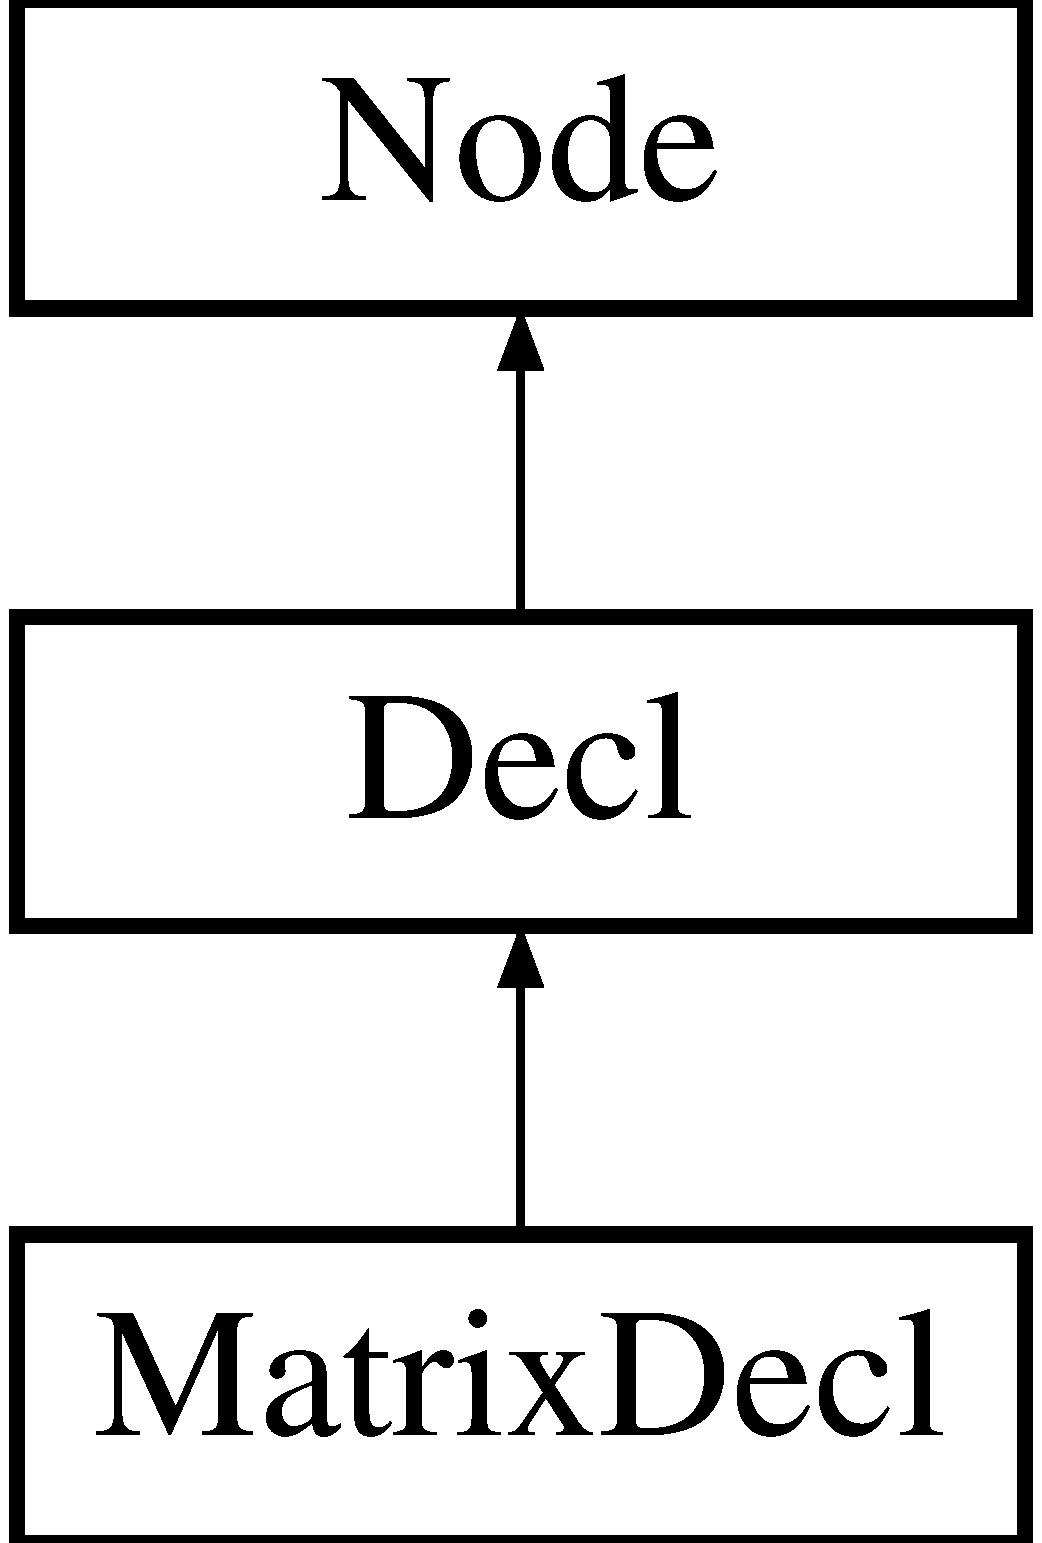
\includegraphics[height=3.000000cm]{classMatrixDecl}
\end{center}
\end{figure}
\subsection*{Additional Inherited Members}


The documentation for this class was generated from the following file\-:\begin{DoxyCompactItemize}
\item 
A\-S\-T.\-h\end{DoxyCompactItemize}

\hypertarget{classNode}{\section{Node Class Reference}
\label{classNode}\index{Node@{Node}}
}
Inheritance diagram for Node\-:\begin{figure}[H]
\begin{center}
\leavevmode
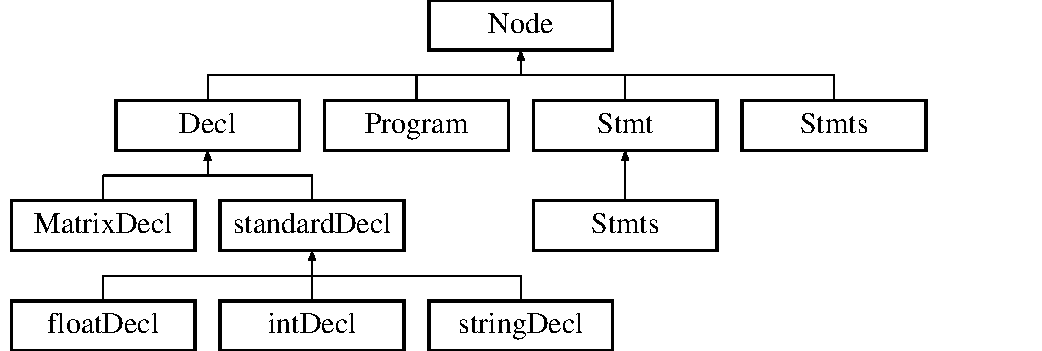
\includegraphics[height=4.000000cm]{classNode}
\end{center}
\end{figure}
\subsection*{Public Member Functions}
\begin{DoxyCompactItemize}
\item 
\hypertarget{classNode_aeb327c708aa4acd82d0f11a9620f0ae8}{virtual std\-::string {\bfseries unparse} ()}\label{classNode_aeb327c708aa4acd82d0f11a9620f0ae8}

\item 
\hypertarget{classNode_ab9dc8a0791d329231bc8427a7d7e9c2f}{virtual std\-::string {\bfseries cpp\-Code} ()}\label{classNode_ab9dc8a0791d329231bc8427a7d7e9c2f}

\end{DoxyCompactItemize}


The documentation for this class was generated from the following file\-:\begin{DoxyCompactItemize}
\item 
A\-S\-T.\-h\end{DoxyCompactItemize}

\hypertarget{classNotOpToken}{\section{Not\-Op\-Token Class Reference}
\label{classNotOpToken}\index{Not\-Op\-Token@{Not\-Op\-Token}}
}
Inheritance diagram for Not\-Op\-Token\-:\begin{figure}[H]
\begin{center}
\leavevmode
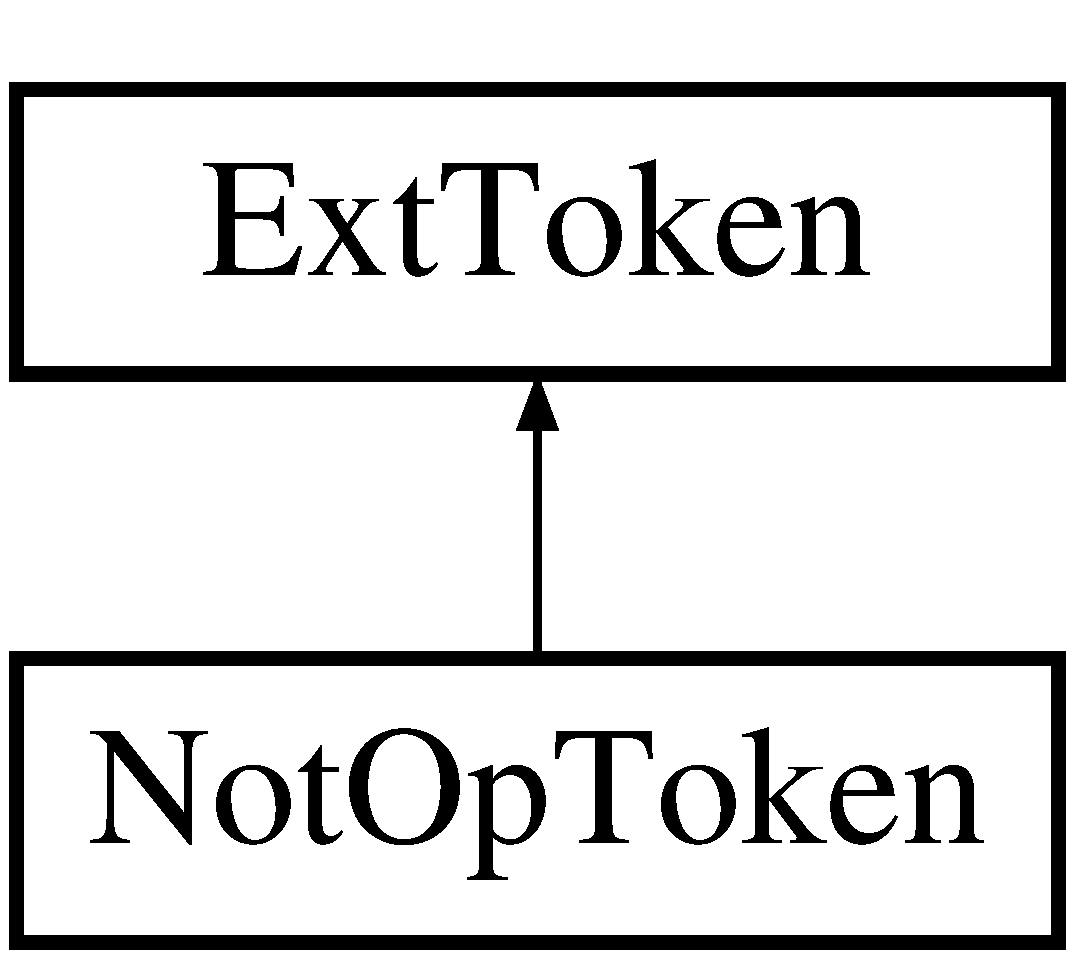
\includegraphics[height=2.000000cm]{classNotOpToken}
\end{center}
\end{figure}
\subsection*{Public Member Functions}
\begin{DoxyCompactItemize}
\item 
\hypertarget{classNotOpToken_afb8b9e96a178b1dfd69abf0a901dfddf}{{\bfseries Not\-Op\-Token} (\hyperlink{classParser}{Parser} $\ast$p, \hyperlink{classToken}{Token} $\ast$t)}\label{classNotOpToken_afb8b9e96a178b1dfd69abf0a901dfddf}

\item 
\hypertarget{classNotOpToken_a55a0dd53742aaca04338c16be079b031}{\hyperlink{classParseResult}{Parse\-Result} {\bfseries nud} ()}\label{classNotOpToken_a55a0dd53742aaca04338c16be079b031}

\item 
\hypertarget{classNotOpToken_a136a11f1e42542a9a58b7c14249c9d23}{std\-::string {\bfseries description} ()}\label{classNotOpToken_a136a11f1e42542a9a58b7c14249c9d23}

\end{DoxyCompactItemize}
\subsection*{Additional Inherited Members}


The documentation for this class was generated from the following file\-:\begin{DoxyCompactItemize}
\item 
ext\-Token.\-h\end{DoxyCompactItemize}

\hypertarget{classParser}{\section{Parser Class Reference}
\label{classParser}\index{Parser@{Parser}}
}
\subsection*{Public Member Functions}
\begin{DoxyCompactItemize}
\item 
\hypertarget{classParser_a2c1a7aa0b09a43bc1eef460817efb1d6}{\hyperlink{classParseResult}{Parse\-Result} {\bfseries parse} (const char $\ast$text)}\label{classParser_a2c1a7aa0b09a43bc1eef460817efb1d6}

\item 
\hypertarget{classParser_a14e25c84322809e2f060dc530362ea71}{\hyperlink{classParseResult}{Parse\-Result} {\bfseries parse\-Program} ()}\label{classParser_a14e25c84322809e2f060dc530362ea71}

\item 
\hypertarget{classParser_ac646227983887c1cd13dae67fa1bc142}{\hyperlink{classParseResult}{Parse\-Result} {\bfseries parse\-Decl} ()}\label{classParser_ac646227983887c1cd13dae67fa1bc142}

\item 
\hypertarget{classParser_a1e1f83c0f4b11148a356d951f191425e}{\hyperlink{classParseResult}{Parse\-Result} {\bfseries parse\-Standard\-Decl} ()}\label{classParser_a1e1f83c0f4b11148a356d951f191425e}

\item 
\hypertarget{classParser_a3a00df25fda2af308b69f05eed14ac69}{\hyperlink{classParseResult}{Parse\-Result} {\bfseries parse\-Matrix\-Decl} ()}\label{classParser_a3a00df25fda2af308b69f05eed14ac69}

\item 
\hypertarget{classParser_a452db3def31683cb0305e57a01489bd4}{\hyperlink{classParseResult}{Parse\-Result} {\bfseries parse\-Stmts} ()}\label{classParser_a452db3def31683cb0305e57a01489bd4}

\item 
\hypertarget{classParser_a9709c4793d0cce012d595f3ee416cd25}{\hyperlink{classParseResult}{Parse\-Result} {\bfseries parse\-Stmt} ()}\label{classParser_a9709c4793d0cce012d595f3ee416cd25}

\item 
\hypertarget{classParser_a50227dc24dc7a175ac0533d9957dfcf8}{\hyperlink{classParseResult}{Parse\-Result} {\bfseries parse\-Expr} (int rbp)}\label{classParser_a50227dc24dc7a175ac0533d9957dfcf8}

\item 
\hypertarget{classParser_ad40f1e5e4c66814f959d982f94b767a3}{\hyperlink{classParseResult}{Parse\-Result} {\bfseries parse\-True\-Kwd} ()}\label{classParser_ad40f1e5e4c66814f959d982f94b767a3}

\item 
\hypertarget{classParser_a56f03d2e70d12648c55ce56a11e63324}{\hyperlink{classParseResult}{Parse\-Result} {\bfseries parse\-False\-Kwd} ()}\label{classParser_a56f03d2e70d12648c55ce56a11e63324}

\item 
\hypertarget{classParser_a2b200b744e5bedf82ef6f610d7877cfc}{\hyperlink{classParseResult}{Parse\-Result} {\bfseries parse\-Int\-Const} ()}\label{classParser_a2b200b744e5bedf82ef6f610d7877cfc}

\item 
\hypertarget{classParser_aaf7b1176fd53246f59577c7eec8b9d22}{\hyperlink{classParseResult}{Parse\-Result} {\bfseries parse\-Float\-Const} ()}\label{classParser_aaf7b1176fd53246f59577c7eec8b9d22}

\item 
\hypertarget{classParser_a4d8930d45c2b730912154c46cc54833c}{\hyperlink{classParseResult}{Parse\-Result} {\bfseries parse\-String\-Const} ()}\label{classParser_a4d8930d45c2b730912154c46cc54833c}

\item 
\hypertarget{classParser_a49c9b3d31ca060c97873e5485d518da3}{\hyperlink{classParseResult}{Parse\-Result} {\bfseries parse\-Char\-Const} ()}\label{classParser_a49c9b3d31ca060c97873e5485d518da3}

\item 
\hypertarget{classParser_a8c1baf62f71da64590e883e51ce622ca}{\hyperlink{classParseResult}{Parse\-Result} {\bfseries parse\-Variable\-Name} ()}\label{classParser_a8c1baf62f71da64590e883e51ce622ca}

\item 
\hypertarget{classParser_aec4c38e1e63c9becfd3a8fc4a1a73f01}{\hyperlink{classParseResult}{Parse\-Result} {\bfseries parse\-Nested\-Expr} ()}\label{classParser_aec4c38e1e63c9becfd3a8fc4a1a73f01}

\item 
\hypertarget{classParser_a1503ceff46112d6d4f0e01b5fb77afcd}{\hyperlink{classParseResult}{Parse\-Result} {\bfseries parse\-Not\-Expr} ()}\label{classParser_a1503ceff46112d6d4f0e01b5fb77afcd}

\item 
\hypertarget{classParser_aa24c33b04779801b330d7fe5a74349e5}{\hyperlink{classParseResult}{Parse\-Result} {\bfseries parse\-Let\-Expr} ()}\label{classParser_aa24c33b04779801b330d7fe5a74349e5}

\item 
\hypertarget{classParser_a555bc6f671d408208e6d049f8e9f3c86}{\hyperlink{classParseResult}{Parse\-Result} {\bfseries parse\-If\-Expr} ()}\label{classParser_a555bc6f671d408208e6d049f8e9f3c86}

\item 
\hypertarget{classParser_ae09cb2b5a7f80c6ad4ad9ccf27a746ca}{\hyperlink{classParseResult}{Parse\-Result} {\bfseries parse\-Addition} (\hyperlink{classParseResult}{Parse\-Result} left)}\label{classParser_ae09cb2b5a7f80c6ad4ad9ccf27a746ca}

\item 
\hypertarget{classParser_a52e6a57d53fc98e5819cc51b3cbe5bd5}{\hyperlink{classParseResult}{Parse\-Result} {\bfseries parse\-Multiplication} (\hyperlink{classParseResult}{Parse\-Result} left)}\label{classParser_a52e6a57d53fc98e5819cc51b3cbe5bd5}

\item 
\hypertarget{classParser_ac22cf1f77e0ca4c23942d5cbcc47eb37}{\hyperlink{classParseResult}{Parse\-Result} {\bfseries parse\-Subtraction} (\hyperlink{classParseResult}{Parse\-Result} left)}\label{classParser_ac22cf1f77e0ca4c23942d5cbcc47eb37}

\item 
\hypertarget{classParser_ad05e6cd1bf83179ecb727b83cbbd0c4e}{\hyperlink{classParseResult}{Parse\-Result} {\bfseries parse\-Division} (\hyperlink{classParseResult}{Parse\-Result} left)}\label{classParser_ad05e6cd1bf83179ecb727b83cbbd0c4e}

\item 
\hypertarget{classParser_ab42ecabc4dbe601d5ed9667351c0c0b8}{\hyperlink{classParseResult}{Parse\-Result} {\bfseries parse\-Relational\-Expr} (\hyperlink{classParseResult}{Parse\-Result} left)}\label{classParser_ab42ecabc4dbe601d5ed9667351c0c0b8}

\item 
\hypertarget{classParser_a3199aab5275c8b6477245eb866fabf35}{void {\bfseries match} (token\-Type tt)}\label{classParser_a3199aab5275c8b6477245eb866fabf35}

\item 
\hypertarget{classParser_a151ffb920a67527813d77bc4ba44c4a7}{bool {\bfseries attempt\-Match} (token\-Type tt)}\label{classParser_a151ffb920a67527813d77bc4ba44c4a7}

\item 
\hypertarget{classParser_a67a10b685bd263477b5f59f1923cdec3}{bool {\bfseries next\-Is} (token\-Type tt)}\label{classParser_a67a10b685bd263477b5f59f1923cdec3}

\item 
\hypertarget{classParser_a324a5bb61c9dfc645300a92aecd6fe69}{void {\bfseries next\-Token} ()}\label{classParser_a324a5bb61c9dfc645300a92aecd6fe69}

\item 
\hypertarget{classParser_a1f45059a13bc0c98355278a9ca9feed9}{std\-::string {\bfseries terminal\-Description} (token\-Type terminal)}\label{classParser_a1f45059a13bc0c98355278a9ca9feed9}

\item 
\hypertarget{classParser_a341bee73e8b1e8558505a237846b16b3}{std\-::string {\bfseries make\-Error\-Msg} (token\-Type terminal)}\label{classParser_a341bee73e8b1e8558505a237846b16b3}

\item 
\hypertarget{classParser_ad38e58ddee85db2aecbd3c7bdcf42116}{std\-::string {\bfseries make\-Error\-Msg\-Expected} (token\-Type terminal)}\label{classParser_ad38e58ddee85db2aecbd3c7bdcf42116}

\item 
\hypertarget{classParser_a60c23daeffb7ced92599e4f2555f71c9}{std\-::string {\bfseries make\-Error\-Msg} (const char $\ast$msg)}\label{classParser_a60c23daeffb7ced92599e4f2555f71c9}

\end{DoxyCompactItemize}
\subsection*{Public Attributes}
\begin{DoxyCompactItemize}
\item 
\hypertarget{classParser_a3606ff327be18af7f76df95f50851633}{\hyperlink{classExtToken}{Ext\-Token} $\ast$ {\bfseries tokens}}\label{classParser_a3606ff327be18af7f76df95f50851633}

\item 
\hypertarget{classParser_a75ab2e2b9385c14e5f967f873340ed11}{\hyperlink{classExtToken}{Ext\-Token} $\ast$ {\bfseries curr\-Token}}\label{classParser_a75ab2e2b9385c14e5f967f873340ed11}

\item 
\hypertarget{classParser_a4bcf7560a5ea1b486bbe4bb54a5a22eb}{\hyperlink{classExtToken}{Ext\-Token} $\ast$ {\bfseries prev\-Token}}\label{classParser_a4bcf7560a5ea1b486bbe4bb54a5a22eb}

\item 
\hypertarget{classParser_a0910de176dcc1cdfbf7ad99622ce9dd5}{\hyperlink{classToken}{Token} $\ast$ {\bfseries stokens}}\label{classParser_a0910de176dcc1cdfbf7ad99622ce9dd5}

\item 
\hypertarget{classParser_ab2ef99ea9e732f5fd176b3949a6c32af}{\hyperlink{classScanner}{Scanner} $\ast$ {\bfseries s}}\label{classParser_ab2ef99ea9e732f5fd176b3949a6c32af}

\end{DoxyCompactItemize}


The documentation for this class was generated from the following files\-:\begin{DoxyCompactItemize}
\item 
parser.\-h\item 
parser.\-cpp\end{DoxyCompactItemize}

\hypertarget{classParseResult}{\section{Parse\-Result Class Reference}
\label{classParseResult}\index{Parse\-Result@{Parse\-Result}}
}
\subsection*{Public Attributes}
\begin{DoxyCompactItemize}
\item 
\hypertarget{classParseResult_ab2dd8deb95c5177148f488ca5d31307a}{std\-::string {\bfseries errors}}\label{classParseResult_ab2dd8deb95c5177148f488ca5d31307a}

\item 
\hypertarget{classParseResult_aa04c6ed3cba109f276e5bc089ca2ff15}{\hyperlink{classNode}{Node} $\ast$ {\bfseries ast}}\label{classParseResult_aa04c6ed3cba109f276e5bc089ca2ff15}

\item 
\hypertarget{classParseResult_a64eb6658c1fc5bbf35fdce181f6845d5}{bool {\bfseries ok}}\label{classParseResult_a64eb6658c1fc5bbf35fdce181f6845d5}

\end{DoxyCompactItemize}


The documentation for this class was generated from the following files\-:\begin{DoxyCompactItemize}
\item 
parse\-Result.\-h\item 
parse\-Result.\-cpp\end{DoxyCompactItemize}

\hypertarget{classParserTestSuite}{\section{Parser\-Test\-Suite Class Reference}
\label{classParserTestSuite}\index{Parser\-Test\-Suite@{Parser\-Test\-Suite}}
}
Inheritance diagram for Parser\-Test\-Suite\-:\begin{figure}[H]
\begin{center}
\leavevmode
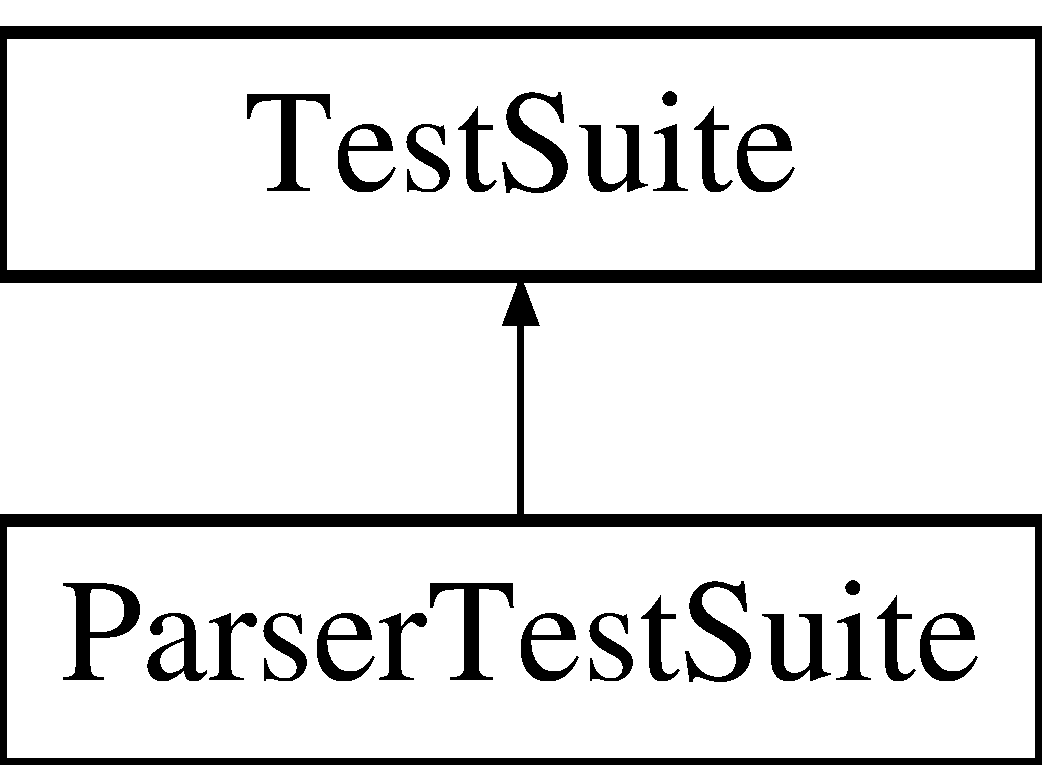
\includegraphics[height=2.000000cm]{classParserTestSuite}
\end{center}
\end{figure}
\subsection*{Public Member Functions}
\begin{DoxyCompactItemize}
\item 
\hypertarget{classParserTestSuite_ab7eff3217b5e28c9003f27c51da107ac}{void {\bfseries test\-\_\-setup\-\_\-code} ()}\label{classParserTestSuite_ab7eff3217b5e28c9003f27c51da107ac}

\item 
\hypertarget{classParserTestSuite_ac4a829a66a1582bee38e90ac3f0355f4}{void {\bfseries test\-\_\-parse\-\_\-bad\-\_\-syntax} ()}\label{classParserTestSuite_ac4a829a66a1582bee38e90ac3f0355f4}

\item 
\hypertarget{classParserTestSuite_a26eed485bc2671f4ac256ef97a21b704}{void {\bfseries test\-\_\-parse\-\_\-sample\-\_\-1} ()}\label{classParserTestSuite_a26eed485bc2671f4ac256ef97a21b704}

\item 
\hypertarget{classParserTestSuite_a0f1d6af1e07e35541fb83416d5e3e229}{void {\bfseries test\-\_\-parse\-\_\-sample\-\_\-2} ()}\label{classParserTestSuite_a0f1d6af1e07e35541fb83416d5e3e229}

\item 
\hypertarget{classParserTestSuite_aecc132f6b6dbb2e5bba08baec64f3f65}{void {\bfseries test\-\_\-parse\-\_\-sample\-\_\-3} ()}\label{classParserTestSuite_aecc132f6b6dbb2e5bba08baec64f3f65}

\item 
\hypertarget{classParserTestSuite_a6e5dfaf7b8ddc98001a4fec39b3f0a79}{void {\bfseries test\-\_\-parse\-\_\-sample\-\_\-4} ()}\label{classParserTestSuite_a6e5dfaf7b8ddc98001a4fec39b3f0a79}

\item 
\hypertarget{classParserTestSuite_a5b9a3cf2b76271244baaaaa4c8b7f7d5}{void {\bfseries test\-\_\-parse\-\_\-sample\-\_\-5} ()}\label{classParserTestSuite_a5b9a3cf2b76271244baaaaa4c8b7f7d5}

\item 
\hypertarget{classParserTestSuite_ae59d0f6d92f8d83833d51ef01479fdeb}{void {\bfseries test\-\_\-parse\-\_\-mysample} ()}\label{classParserTestSuite_ae59d0f6d92f8d83833d51ef01479fdeb}

\item 
\hypertarget{classParserTestSuite_a379db1a22b2c32defb8395b9b2166f76}{void {\bfseries test\-\_\-parse\-\_\-forest\-Loss\-V2} ()}\label{classParserTestSuite_a379db1a22b2c32defb8395b9b2166f76}

\end{DoxyCompactItemize}
\subsection*{Public Attributes}
\begin{DoxyCompactItemize}
\item 
\hypertarget{classParserTestSuite_a0c4943b3d23b79be363ba9e1ac7c02ed}{\hyperlink{classScanner}{Scanner} $\ast$ {\bfseries s}}\label{classParserTestSuite_a0c4943b3d23b79be363ba9e1ac7c02ed}

\item 
\hypertarget{classParserTestSuite_a1d637f2f8be1326423ee5b4fd270c553}{\hyperlink{classParser}{Parser} $\ast$ {\bfseries p}}\label{classParserTestSuite_a1d637f2f8be1326423ee5b4fd270c553}

\end{DoxyCompactItemize}


The documentation for this class was generated from the following file\-:\begin{DoxyCompactItemize}
\item 
parser\-\_\-tests.\-h\end{DoxyCompactItemize}

\hypertarget{classPlusSignToken}{\section{Plus\-Sign\-Token Class Reference}
\label{classPlusSignToken}\index{Plus\-Sign\-Token@{Plus\-Sign\-Token}}
}
Inheritance diagram for Plus\-Sign\-Token\-:\begin{figure}[H]
\begin{center}
\leavevmode
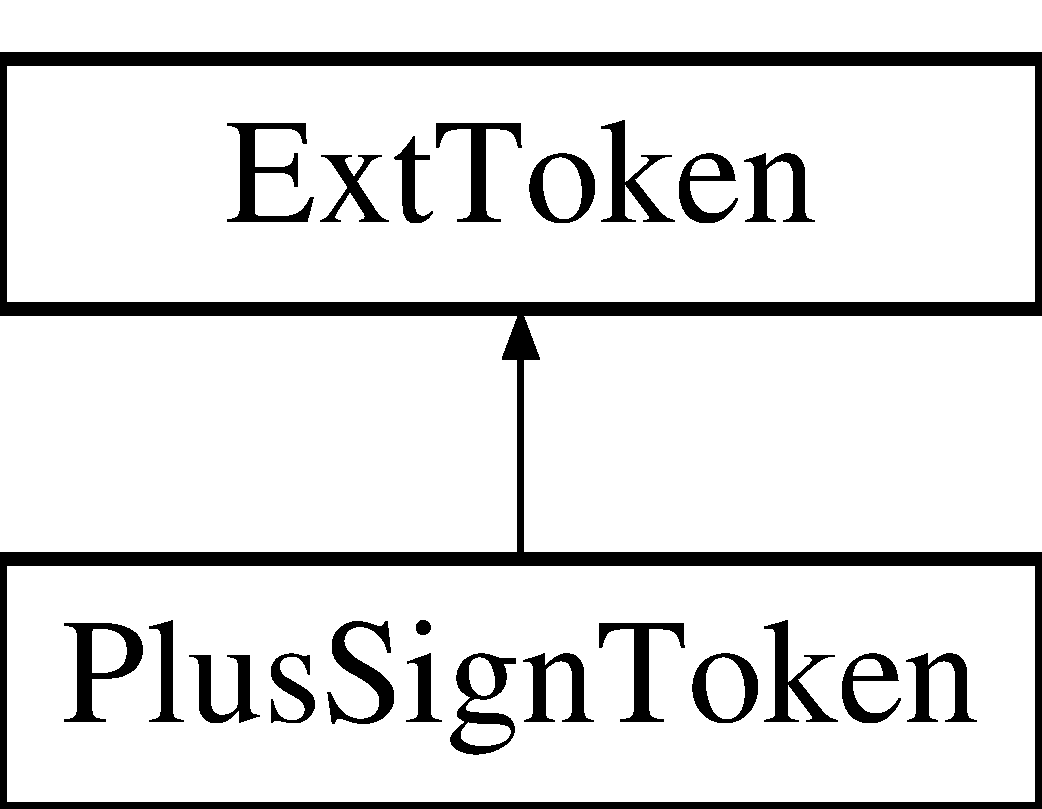
\includegraphics[height=2.000000cm]{classPlusSignToken}
\end{center}
\end{figure}
\subsection*{Public Member Functions}
\begin{DoxyCompactItemize}
\item 
\hypertarget{classPlusSignToken_ad480457c426f911f8286a73e8cf7f949}{{\bfseries Plus\-Sign\-Token} (\hyperlink{classParser}{Parser} $\ast$p, \hyperlink{classToken}{Token} $\ast$t)}\label{classPlusSignToken_ad480457c426f911f8286a73e8cf7f949}

\item 
\hypertarget{classPlusSignToken_a4d79a17891f92800259308ce71402526}{\hyperlink{classParseResult}{Parse\-Result} {\bfseries led} (\hyperlink{classParseResult}{Parse\-Result} left)}\label{classPlusSignToken_a4d79a17891f92800259308ce71402526}

\item 
\hypertarget{classPlusSignToken_a61a05ac9660848e13da97d5746808868}{std\-::string {\bfseries description} ()}\label{classPlusSignToken_a61a05ac9660848e13da97d5746808868}

\item 
\hypertarget{classPlusSignToken_a80753eec970928e042da350df83150f2}{int {\bfseries lbp} ()}\label{classPlusSignToken_a80753eec970928e042da350df83150f2}

\end{DoxyCompactItemize}
\subsection*{Additional Inherited Members}


The documentation for this class was generated from the following file\-:\begin{DoxyCompactItemize}
\item 
ext\-Token.\-h\end{DoxyCompactItemize}

\hypertarget{classProgram}{\section{Program Class Reference}
\label{classProgram}\index{Program@{Program}}
}
Inheritance diagram for Program\-:\begin{figure}[H]
\begin{center}
\leavevmode
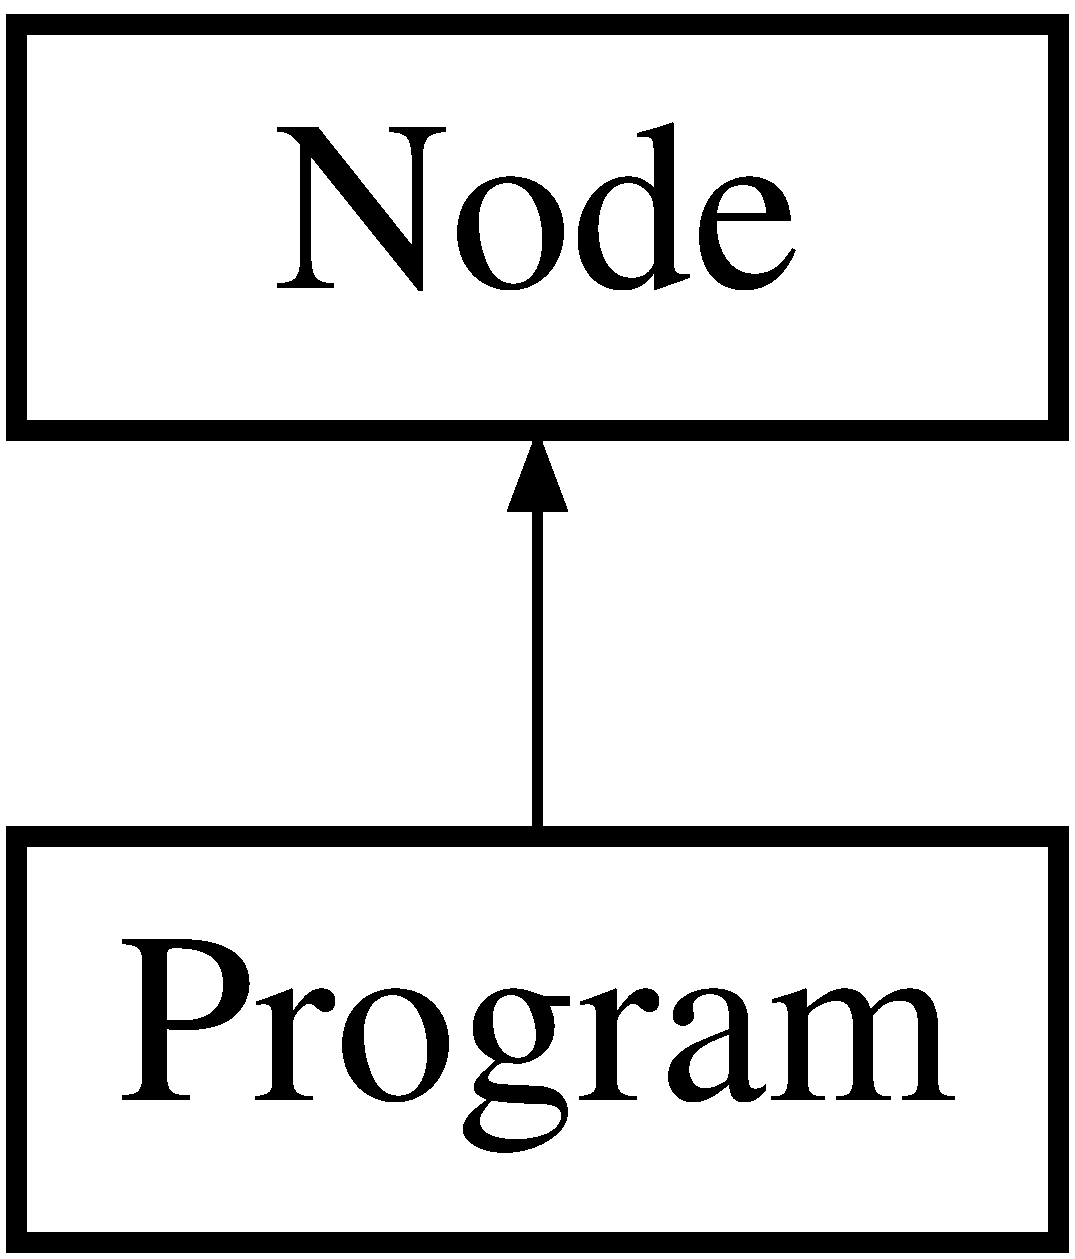
\includegraphics[height=2.000000cm]{classProgram}
\end{center}
\end{figure}
\subsection*{Additional Inherited Members}


The documentation for this class was generated from the following file\-:\begin{DoxyCompactItemize}
\item 
A\-S\-T.\-h\end{DoxyCompactItemize}

\hypertarget{classRegexTestSuite}{\section{Regex\-Test\-Suite Class Reference}
\label{classRegexTestSuite}\index{Regex\-Test\-Suite@{Regex\-Test\-Suite}}
}
Inheritance diagram for Regex\-Test\-Suite\-:\begin{figure}[H]
\begin{center}
\leavevmode
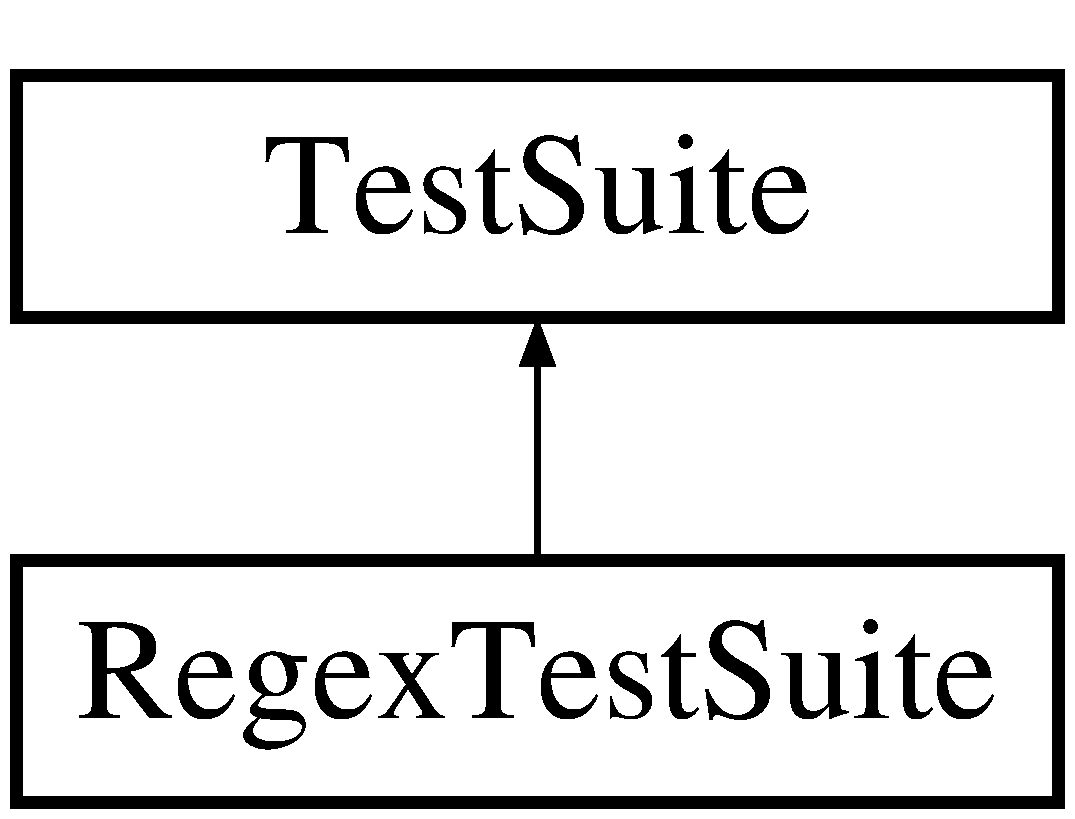
\includegraphics[height=2.000000cm]{classRegexTestSuite}
\end{center}
\end{figure}
\subsection*{Public Member Functions}
\begin{DoxyCompactItemize}
\item 
\hypertarget{classRegexTestSuite_aac0838d917fd9fd6cc71ee086c644555}{void {\bfseries test\-\_\-make\-\_\-match\-Regex\-\_\-match} (void)}\label{classRegexTestSuite_aac0838d917fd9fd6cc71ee086c644555}

\item 
\hypertarget{classRegexTestSuite_ad9c02b9f4fd7feca750d476cda8e0c60}{void {\bfseries test\-\_\-make\-\_\-match\-Regex\-\_\-no\-\_\-match} (void)}\label{classRegexTestSuite_ad9c02b9f4fd7feca750d476cda8e0c60}

\item 
\hypertarget{classRegexTestSuite_a0f46b90e2c0a1c98750a3335d086979a}{void {\bfseries test\-\_\-make\-\_\-match\-Regex\-\_\-match\-\_\-string\-\_\-copy} (void)}\label{classRegexTestSuite_a0f46b90e2c0a1c98750a3335d086979a}

\end{DoxyCompactItemize}


The documentation for this class was generated from the following file\-:\begin{DoxyCompactItemize}
\item 
regex\-\_\-tests.\-h\end{DoxyCompactItemize}

\hypertarget{classRelationalOpToken}{\section{Relational\-Op\-Token Class Reference}
\label{classRelationalOpToken}\index{Relational\-Op\-Token@{Relational\-Op\-Token}}
}
Inheritance diagram for Relational\-Op\-Token\-:\begin{figure}[H]
\begin{center}
\leavevmode
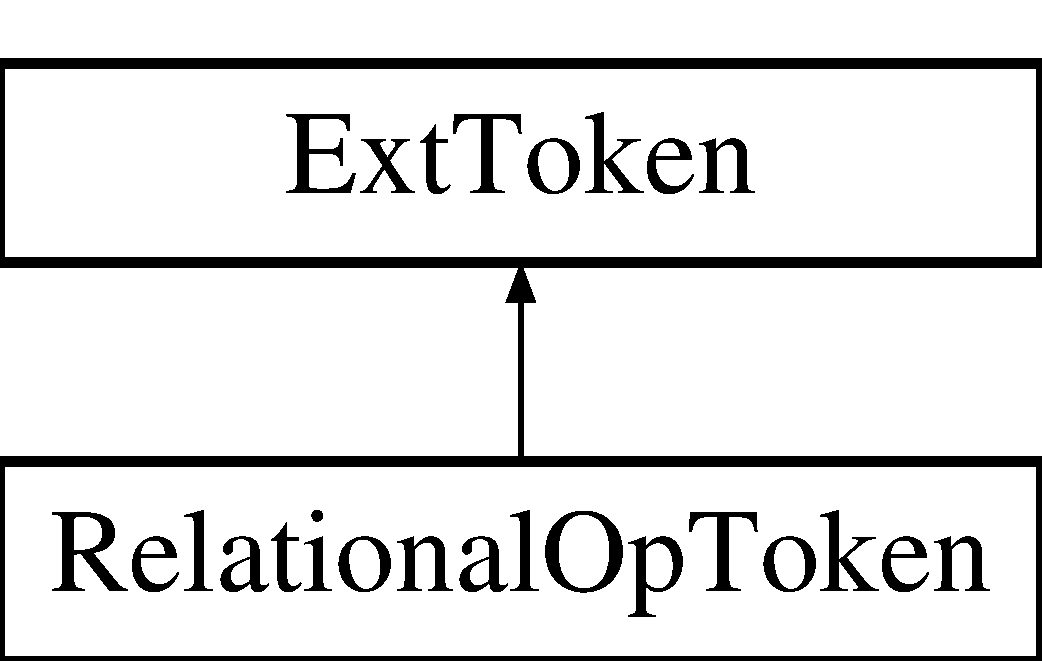
\includegraphics[height=2.000000cm]{classRelationalOpToken}
\end{center}
\end{figure}
\subsection*{Public Member Functions}
\begin{DoxyCompactItemize}
\item 
\hypertarget{classRelationalOpToken_a1ede45cf178138ff12beba209681be51}{{\bfseries Relational\-Op\-Token} (\hyperlink{classParser}{Parser} $\ast$p, \hyperlink{classToken}{Token} $\ast$t, std\-::string d)}\label{classRelationalOpToken_a1ede45cf178138ff12beba209681be51}

\item 
\hypertarget{classRelationalOpToken_a426c64391e7b3272d8e6277964730e05}{\hyperlink{classParseResult}{Parse\-Result} {\bfseries led} (\hyperlink{classParseResult}{Parse\-Result} left)}\label{classRelationalOpToken_a426c64391e7b3272d8e6277964730e05}

\item 
\hypertarget{classRelationalOpToken_ada096491d9553aea21089230489d6aef}{int {\bfseries lbp} ()}\label{classRelationalOpToken_ada096491d9553aea21089230489d6aef}

\end{DoxyCompactItemize}
\subsection*{Additional Inherited Members}


The documentation for this class was generated from the following file\-:\begin{DoxyCompactItemize}
\item 
ext\-Token.\-h\end{DoxyCompactItemize}

\hypertarget{classScanner}{\section{Scanner Class Reference}
\label{classScanner}\index{Scanner@{Scanner}}
}
\subsection*{Public Member Functions}
\begin{DoxyCompactItemize}
\item 
\hypertarget{classScanner_a289dc1f278cdea9c7f290ad46cf85bd2}{{\bfseries Scanner} (\hyperlink{classToken}{Token} $\ast$toke)}\label{classScanner_a289dc1f278cdea9c7f290ad46cf85bd2}

\item 
\hypertarget{classScanner_a186ae0ef8cd6cd6ef6c78d670c1fabaf}{void {\bfseries push} (\hyperlink{classToken}{Token} $\ast$toke)}\label{classScanner_a186ae0ef8cd6cd6ef6c78d670c1fabaf}

\item 
\hypertarget{classScanner_ab2957742ec855cce79d1fadc4eafc8c0}{\hyperlink{classToken}{Token} $\ast$ {\bfseries pop} ()}\label{classScanner_ab2957742ec855cce79d1fadc4eafc8c0}

\item 
\hypertarget{classScanner_aa73c3f66ddedf18b0b6f096bffaabbfa}{\hyperlink{classToken}{Token} $\ast$ {\bfseries get\-Head} ()}\label{classScanner_aa73c3f66ddedf18b0b6f096bffaabbfa}

\item 
\hypertarget{classScanner_ad991d05bd22fbf1d8eb670bb69eb0460}{void {\bfseries get\-Regx} ()}\label{classScanner_ad991d05bd22fbf1d8eb670bb69eb0460}

\item 
\hypertarget{classScanner_a85e45b51ff72e5515e53609e06d579ca}{\hyperlink{classToken}{Token} $\ast$ {\bfseries make\-Toke} (std\-::string)}\label{classScanner_a85e45b51ff72e5515e53609e06d579ca}

\item 
\hypertarget{classScanner_ad9c3562dc3be00426f9254846605ebda}{\hyperlink{classToken}{Token} $\ast$ {\bfseries make\-Token} (const char $\ast$)}\label{classScanner_ad9c3562dc3be00426f9254846605ebda}

\item 
\hypertarget{classScanner_a4cf90c9e68bfb17f23af7368ff15766e}{\hyperlink{classToken}{Token} $\ast$ {\bfseries scan} (const char $\ast$)}\label{classScanner_a4cf90c9e68bfb17f23af7368ff15766e}

\end{DoxyCompactItemize}
\subsection*{Public Attributes}
\begin{DoxyCompactItemize}
\item 
\hypertarget{classScanner_a238d14dc6c85e8418e2a21a72f3d2a9a}{\hyperlink{classToken}{Token} $\ast$ {\bfseries head}}\label{classScanner_a238d14dc6c85e8418e2a21a72f3d2a9a}

\item 
\hypertarget{classScanner_aa1250cba137879ad6831185650d0641a}{\hyperlink{classToken}{Token} $\ast$ {\bfseries tail}}\label{classScanner_aa1250cba137879ad6831185650d0641a}

\item 
\hypertarget{classScanner_a9c0882c3e4c4e83da0e66bf97aebed19}{regex\-\_\-t $\ast$ {\bfseries regx} \mbox{[}M\-A\-X\-K\-W\-D\-S\mbox{]}}\label{classScanner_a9c0882c3e4c4e83da0e66bf97aebed19}

\end{DoxyCompactItemize}


The documentation for this class was generated from the following files\-:\begin{DoxyCompactItemize}
\item 
scanner.\-h\item 
scanner.\-cpp\end{DoxyCompactItemize}

\hypertarget{classScannerTestSuite}{\section{Scanner\-Test\-Suite Class Reference}
\label{classScannerTestSuite}\index{Scanner\-Test\-Suite@{Scanner\-Test\-Suite}}
}
Inheritance diagram for Scanner\-Test\-Suite\-:\begin{figure}[H]
\begin{center}
\leavevmode
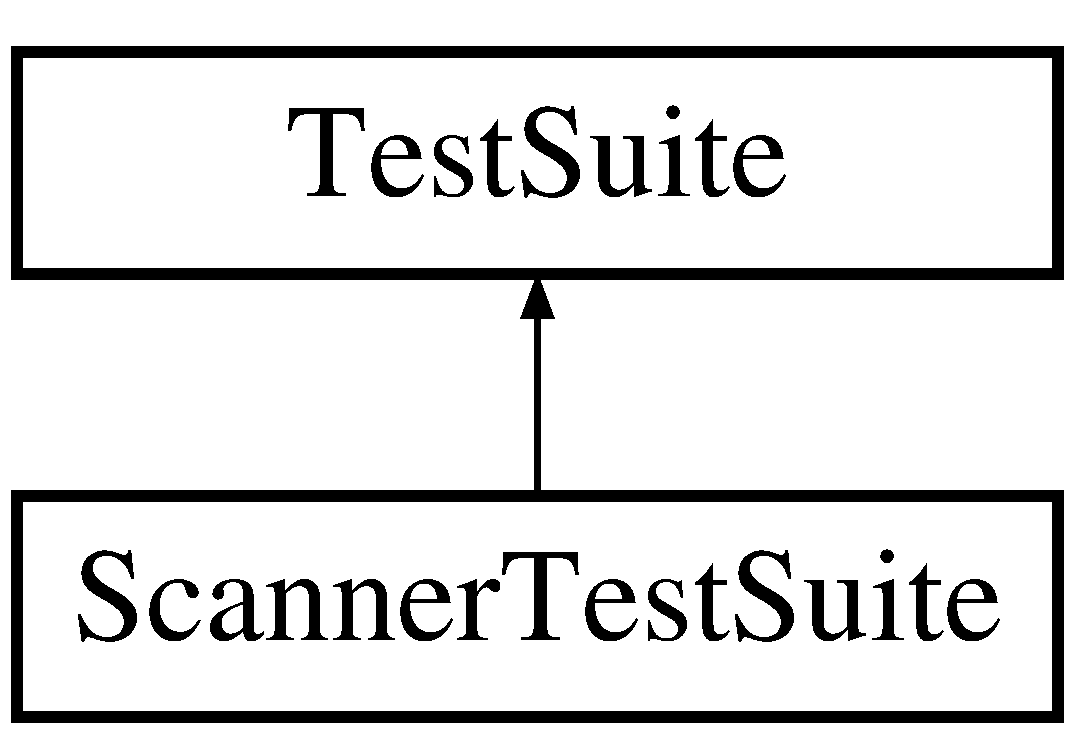
\includegraphics[height=2.000000cm]{classScannerTestSuite}
\end{center}
\end{figure}
\subsection*{Public Member Functions}
\begin{DoxyCompactItemize}
\item 
\hypertarget{classScannerTestSuite_ade832b9b4b3bd92980d43c4050cebd2c}{void {\bfseries test\-\_\-setup\-\_\-code} ()}\label{classScannerTestSuite_ade832b9b4b3bd92980d43c4050cebd2c}

\item 
\hypertarget{classScannerTestSuite_a681db679ec2418f862f478fa7678942b}{bool {\bfseries no\-Lexical\-Errors} (\hyperlink{classToken}{Token} $\ast$tks)}\label{classScannerTestSuite_a681db679ec2418f862f478fa7678942b}

\item 
\hypertarget{classScannerTestSuite_a01dc6065a02127accc049627ae234129}{void {\bfseries scan\-File\-No\-Lexical\-Errors} (const char $\ast$filename)}\label{classScannerTestSuite_a01dc6065a02127accc049627ae234129}

\item 
\hypertarget{classScannerTestSuite_a97c50725866b3a5b36c36488053a59bc}{bool {\bfseries same\-Terminals} (\hyperlink{classToken}{Token} $\ast$tks, int num\-Terms, token\-Type $\ast$ts)}\label{classScannerTestSuite_a97c50725866b3a5b36c36488053a59bc}

\item 
\hypertarget{classScannerTestSuite_a01beafb44a33f4d80baf9a4208919c07}{void {\bfseries test\-\_\-scan\-\_\-empty} ()}\label{classScannerTestSuite_a01beafb44a33f4d80baf9a4208919c07}

\item 
\hypertarget{classScannerTestSuite_a304719dd961df0714d372010cdf99ef1}{void {\bfseries test\-\_\-scan\-\_\-empty\-\_\-comment} ()}\label{classScannerTestSuite_a304719dd961df0714d372010cdf99ef1}

\item 
\hypertarget{classScannerTestSuite_af85168e66ba2b924488aca9768231367}{void {\bfseries test\-\_\-scan\-\_\-lexical\-Errors} ()}\label{classScannerTestSuite_af85168e66ba2b924488aca9768231367}

\item 
\hypertarget{classScannerTestSuite_a4bd4d5fc2218f3d28b08b2821ecc271b}{void {\bfseries test\-\_\-scan\-\_\-nums\-\_\-vars} ()}\label{classScannerTestSuite_a4bd4d5fc2218f3d28b08b2821ecc271b}

\item 
\hypertarget{classScannerTestSuite_aad7648d262ef3c103f0792ef73aa3bd8}{void {\bfseries test\-\_\-scan\-\_\-bad\-\_\-syntax\-\_\-good\-\_\-tokens} ()}\label{classScannerTestSuite_aad7648d262ef3c103f0792ef73aa3bd8}

\item 
\hypertarget{classScannerTestSuite_a8248f8bda6c9909971ef13f1364ab8f8}{void {\bfseries test\-\_\-scan\-\_\-sample\-\_\-forest\-Loss} ()}\label{classScannerTestSuite_a8248f8bda6c9909971ef13f1364ab8f8}

\item 
\hypertarget{classScannerTestSuite_a85d91624b470d65d466390110d74ab99}{void {\bfseries token\-Maker\-\_\-test} (string line, token\-Type terminal, string lexeme)}\label{classScannerTestSuite_a85d91624b470d65d466390110d74ab99}

\item 
\hypertarget{classScannerTestSuite_afd03fbc31003d1be155fba2a3c98b71c}{void {\bfseries test\-\_\-\-Token\-Maker\-\_\-int\-Kwd} ()}\label{classScannerTestSuite_afd03fbc31003d1be155fba2a3c98b71c}

\item 
\hypertarget{classScannerTestSuite_a78fc1b6a686d36de0d9653aaddf4ad88}{void {\bfseries test\-\_\-\-Token\-Maker\-\_\-float\-Kwd} ()}\label{classScannerTestSuite_a78fc1b6a686d36de0d9653aaddf4ad88}

\item 
\hypertarget{classScannerTestSuite_a816712d2c5ec0ef7ef3361dc5a80eb51}{void {\bfseries test\-\_\-\-Token\-Maker\-\_\-bool\-Kwd} ()}\label{classScannerTestSuite_a816712d2c5ec0ef7ef3361dc5a80eb51}

\item 
\hypertarget{classScannerTestSuite_aa9d32f82e08ccc810fca495f4628c2a7}{void {\bfseries test\-\_\-\-Token\-Maker\-\_\-true\-Kwd} ()}\label{classScannerTestSuite_aa9d32f82e08ccc810fca495f4628c2a7}

\item 
\hypertarget{classScannerTestSuite_ab96166b93c96fea8c7e4c5cc44961d39}{void {\bfseries test\-\_\-\-Token\-Maker\-\_\-false\-Kwd} ()}\label{classScannerTestSuite_ab96166b93c96fea8c7e4c5cc44961d39}

\item 
\hypertarget{classScannerTestSuite_a15ec232bf3903ec8527b0a3e37cc443e}{void {\bfseries test\-\_\-\-Token\-Maker\-\_\-string\-Kwd} ()}\label{classScannerTestSuite_a15ec232bf3903ec8527b0a3e37cc443e}

\item 
\hypertarget{classScannerTestSuite_a5d766dff9b08ee580133f042d9e42ea1}{void {\bfseries test\-\_\-\-Token\-Maker\-\_\-matrix\-Kwd} ()}\label{classScannerTestSuite_a5d766dff9b08ee580133f042d9e42ea1}

\item 
\hypertarget{classScannerTestSuite_a6d80c8fac5af9493b09c0cafa42191bf}{void {\bfseries test\-\_\-\-Token\-Maker\-\_\-let\-Kwd} ()}\label{classScannerTestSuite_a6d80c8fac5af9493b09c0cafa42191bf}

\item 
\hypertarget{classScannerTestSuite_a8e25d2acae63b70ed01f2b59e679c92c}{void {\bfseries test\-\_\-\-Token\-Maker\-\_\-in\-Kwd} ()}\label{classScannerTestSuite_a8e25d2acae63b70ed01f2b59e679c92c}

\item 
\hypertarget{classScannerTestSuite_a37ea34a026825d99f924771fa4c22e39}{void {\bfseries test\-\_\-\-Token\-Maker\-\_\-end\-Kwd} ()}\label{classScannerTestSuite_a37ea34a026825d99f924771fa4c22e39}

\item 
\hypertarget{classScannerTestSuite_a967f3d747c68bb95433fcd63d9180051}{void {\bfseries test\-\_\-\-Token\-Maker\-\_\-if\-Kwd} ()}\label{classScannerTestSuite_a967f3d747c68bb95433fcd63d9180051}

\item 
\hypertarget{classScannerTestSuite_af0484460a87be267d9f6faa6897561c4}{void {\bfseries test\-\_\-\-Token\-Maker\-\_\-then\-Kwd} ()}\label{classScannerTestSuite_af0484460a87be267d9f6faa6897561c4}

\item 
\hypertarget{classScannerTestSuite_a7e792719bac6501f55d4e89062d7fa0a}{void {\bfseries test\-\_\-\-Token\-Maker\-\_\-else\-Kwd} ()}\label{classScannerTestSuite_a7e792719bac6501f55d4e89062d7fa0a}

\item 
\hypertarget{classScannerTestSuite_a977f0363e656db5a6df719e4f8e23fd5}{void {\bfseries test\-\_\-\-Token\-Maker\-\_\-for\-Kwd} ()}\label{classScannerTestSuite_a977f0363e656db5a6df719e4f8e23fd5}

\item 
\hypertarget{classScannerTestSuite_a62a89711aa63f71870920fc36a40ab12}{void {\bfseries test\-\_\-\-Token\-Maker\-\_\-while\-Kwd} ()}\label{classScannerTestSuite_a62a89711aa63f71870920fc36a40ab12}

\item 
\hypertarget{classScannerTestSuite_a8f5ccd7ff477d6ee966ae20f1c5f161c}{void {\bfseries test\-\_\-\-Token\-Maker\-\_\-print\-Kwd} ()}\label{classScannerTestSuite_a8f5ccd7ff477d6ee966ae20f1c5f161c}

\item 
\hypertarget{classScannerTestSuite_a5c8d37b6b446f99846356d19ccb9ed05}{void {\bfseries test\-\_\-\-Token\-Maker\-\_\-int\-Const} ()}\label{classScannerTestSuite_a5c8d37b6b446f99846356d19ccb9ed05}

\item 
\hypertarget{classScannerTestSuite_ae3e0058aa6e11470871480461fa2b058}{void {\bfseries test\-\_\-\-Token\-Maker\-\_\-float\-Const} ()}\label{classScannerTestSuite_ae3e0058aa6e11470871480461fa2b058}

\item 
\hypertarget{classScannerTestSuite_a6e95f7c63efa9f7ce519ec2cf557a28d}{void {\bfseries test\-\_\-\-Token\-Maker\-\_\-string\-Const} ()}\label{classScannerTestSuite_a6e95f7c63efa9f7ce519ec2cf557a28d}

\item 
\hypertarget{classScannerTestSuite_af1ebd344911a7fe6065d8bc0f3f53332}{void {\bfseries test\-\_\-\-Token\-Maker\-\_\-variable\-Name} ()}\label{classScannerTestSuite_af1ebd344911a7fe6065d8bc0f3f53332}

\item 
\hypertarget{classScannerTestSuite_a3edc932ed34df7d3f8cf6cefa2da7a00}{void {\bfseries test\-\_\-\-Token\-Maker\-\_\-left\-Paren} ()}\label{classScannerTestSuite_a3edc932ed34df7d3f8cf6cefa2da7a00}

\item 
\hypertarget{classScannerTestSuite_a8e2286c9ba583a40de686a6457577fb1}{void {\bfseries test\-\_\-\-Token\-Maker\-\_\-right\-Paren} ()}\label{classScannerTestSuite_a8e2286c9ba583a40de686a6457577fb1}

\item 
\hypertarget{classScannerTestSuite_a95383cf61a7b55366944fae7147a6dc1}{void {\bfseries test\-\_\-\-Token\-Maker\-\_\-left\-Curly} ()}\label{classScannerTestSuite_a95383cf61a7b55366944fae7147a6dc1}

\item 
\hypertarget{classScannerTestSuite_a844dd609d8a4a89eb128b6634a87107b}{void {\bfseries test\-\_\-\-Token\-Maker\-\_\-right\-Curly} ()}\label{classScannerTestSuite_a844dd609d8a4a89eb128b6634a87107b}

\item 
\hypertarget{classScannerTestSuite_a45b4775dab8fb8d6ca3b6a3b3b53057c}{void {\bfseries test\-\_\-\-Token\-Maker\-\_\-left\-Square} ()}\label{classScannerTestSuite_a45b4775dab8fb8d6ca3b6a3b3b53057c}

\item 
\hypertarget{classScannerTestSuite_ad1bea3188d5ce34f693787fb8a963f55}{void {\bfseries test\-\_\-\-Token\-Maker\-\_\-right\-Square} ()}\label{classScannerTestSuite_ad1bea3188d5ce34f693787fb8a963f55}

\item 
\hypertarget{classScannerTestSuite_a0dadcabb232c6fb73a3bf6f98a6f673b}{void {\bfseries test\-\_\-\-Token\-Maker\-\_\-comma} ()}\label{classScannerTestSuite_a0dadcabb232c6fb73a3bf6f98a6f673b}

\item 
\hypertarget{classScannerTestSuite_ae8bb85e64c0713bc6e37d67ec66407a9}{void {\bfseries test\-\_\-\-Token\-Maker\-\_\-semi\-Colon} ()}\label{classScannerTestSuite_ae8bb85e64c0713bc6e37d67ec66407a9}

\item 
\hypertarget{classScannerTestSuite_af98d5f5c61439723d0cb18f9357d91d8}{void {\bfseries test\-\_\-\-Token\-Maker\-\_\-colon} ()}\label{classScannerTestSuite_af98d5f5c61439723d0cb18f9357d91d8}

\item 
\hypertarget{classScannerTestSuite_aa04a5770dba31012dd42409eebbf0eb8}{void {\bfseries test\-\_\-\-Token\-Maker\-\_\-assign} ()}\label{classScannerTestSuite_aa04a5770dba31012dd42409eebbf0eb8}

\item 
\hypertarget{classScannerTestSuite_ad65fde16b4a37ce6686bbc29b0e42f07}{void {\bfseries test\-\_\-\-Token\-Maker\-\_\-plus\-Sign} ()}\label{classScannerTestSuite_ad65fde16b4a37ce6686bbc29b0e42f07}

\item 
\hypertarget{classScannerTestSuite_af0977bb3ca5ca5954bc787c31b041649}{void {\bfseries test\-\_\-\-Token\-Maker\-\_\-star} ()}\label{classScannerTestSuite_af0977bb3ca5ca5954bc787c31b041649}

\item 
\hypertarget{classScannerTestSuite_a348c6d799fb438215ee94891328f95eb}{void {\bfseries test\-\_\-\-Token\-Maker\-\_\-dash} ()}\label{classScannerTestSuite_a348c6d799fb438215ee94891328f95eb}

\item 
\hypertarget{classScannerTestSuite_a25f1d1c73ad5b607613a34bd5d5c3238}{void {\bfseries test\-\_\-\-Token\-Maker\-\_\-forward\-Slash} ()}\label{classScannerTestSuite_a25f1d1c73ad5b607613a34bd5d5c3238}

\item 
\hypertarget{classScannerTestSuite_afc7124c00488adc7635905290e1159e6}{void {\bfseries test\-\_\-\-Token\-Maker\-\_\-less\-Than} ()}\label{classScannerTestSuite_afc7124c00488adc7635905290e1159e6}

\item 
\hypertarget{classScannerTestSuite_a2b2720fe2932b4db758df6c67e1bef14}{void {\bfseries test\-\_\-\-Token\-Maker\-\_\-less\-Than\-Equal} ()}\label{classScannerTestSuite_a2b2720fe2932b4db758df6c67e1bef14}

\item 
\hypertarget{classScannerTestSuite_a2d3ebde4e350cb1ee4ee8c53c54bf0a0}{void {\bfseries test\-\_\-\-Token\-Maker\-\_\-greater\-Than} ()}\label{classScannerTestSuite_a2d3ebde4e350cb1ee4ee8c53c54bf0a0}

\item 
\hypertarget{classScannerTestSuite_a9805d181580e4b7fafa00b0beaf53a32}{void {\bfseries test\-\_\-\-Token\-Maker\-\_\-greater\-Than\-Equal} ()}\label{classScannerTestSuite_a9805d181580e4b7fafa00b0beaf53a32}

\item 
\hypertarget{classScannerTestSuite_a5a591c0c62d905129744f660ca74149d}{void {\bfseries test\-\_\-\-Token\-Maker\-\_\-equal\-Equals} ()}\label{classScannerTestSuite_a5a591c0c62d905129744f660ca74149d}

\item 
\hypertarget{classScannerTestSuite_a9ee2f76c0deeb7b0c99d1be5d895c46f}{void {\bfseries test\-\_\-\-Token\-Maker\-\_\-not\-Equals} ()}\label{classScannerTestSuite_a9ee2f76c0deeb7b0c99d1be5d895c46f}

\item 
\hypertarget{classScannerTestSuite_aa71ec0de76c1afa02ff6468f60fc188f}{void {\bfseries test\-\_\-\-Token\-Maker\-\_\-and\-Op} ()}\label{classScannerTestSuite_aa71ec0de76c1afa02ff6468f60fc188f}

\item 
\hypertarget{classScannerTestSuite_a79743fed40c2a7e325dab1804c6a863b}{void {\bfseries test\-\_\-\-Token\-Maker\-\_\-or\-Op} ()}\label{classScannerTestSuite_a79743fed40c2a7e325dab1804c6a863b}

\item 
\hypertarget{classScannerTestSuite_ade8c573d5c330cdedca37d3dc61220a7}{void {\bfseries test\-\_\-\-Token\-Maker\-\_\-not\-Op} ()}\label{classScannerTestSuite_ade8c573d5c330cdedca37d3dc61220a7}

\end{DoxyCompactItemize}
\subsection*{Public Attributes}
\begin{DoxyCompactItemize}
\item 
\hypertarget{classScannerTestSuite_a39987f3459098101d7c7fb5a4492996d}{\hyperlink{classScanner}{Scanner} $\ast$ {\bfseries s}}\label{classScannerTestSuite_a39987f3459098101d7c7fb5a4492996d}

\end{DoxyCompactItemize}


The documentation for this class was generated from the following file\-:\begin{DoxyCompactItemize}
\item 
scanner\-\_\-tests.\-h\end{DoxyCompactItemize}

\hypertarget{classstandardDecl}{\section{standard\-Decl Class Reference}
\label{classstandardDecl}\index{standard\-Decl@{standard\-Decl}}
}
Inheritance diagram for standard\-Decl\-:\begin{figure}[H]
\begin{center}
\leavevmode
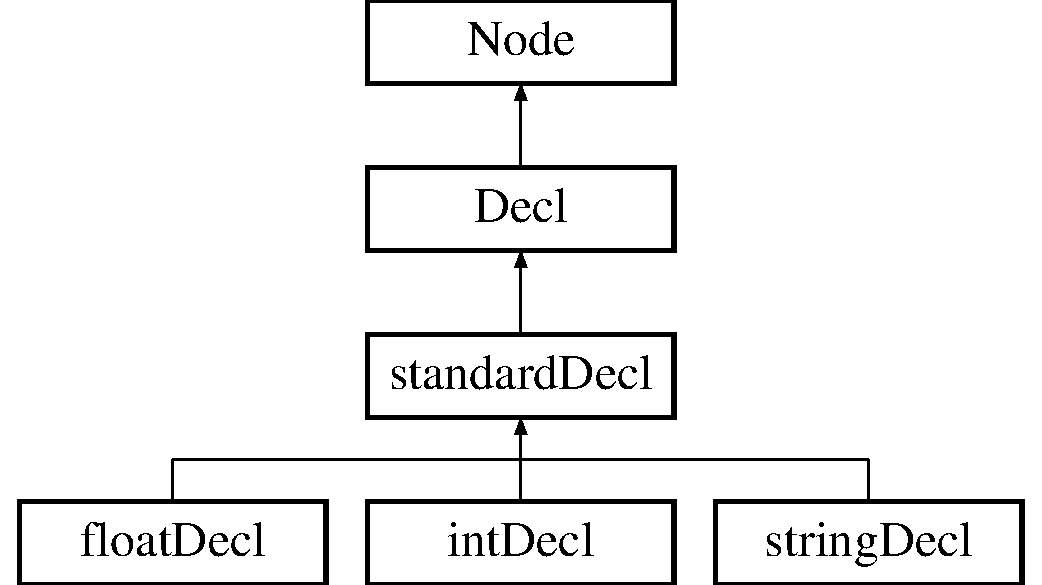
\includegraphics[height=4.000000cm]{classstandardDecl}
\end{center}
\end{figure}
\subsection*{Additional Inherited Members}


The documentation for this class was generated from the following file\-:\begin{DoxyCompactItemize}
\item 
A\-S\-T.\-h\end{DoxyCompactItemize}

\hypertarget{classStarToken}{\section{Star\-Token Class Reference}
\label{classStarToken}\index{Star\-Token@{Star\-Token}}
}
Inheritance diagram for Star\-Token\-:\begin{figure}[H]
\begin{center}
\leavevmode
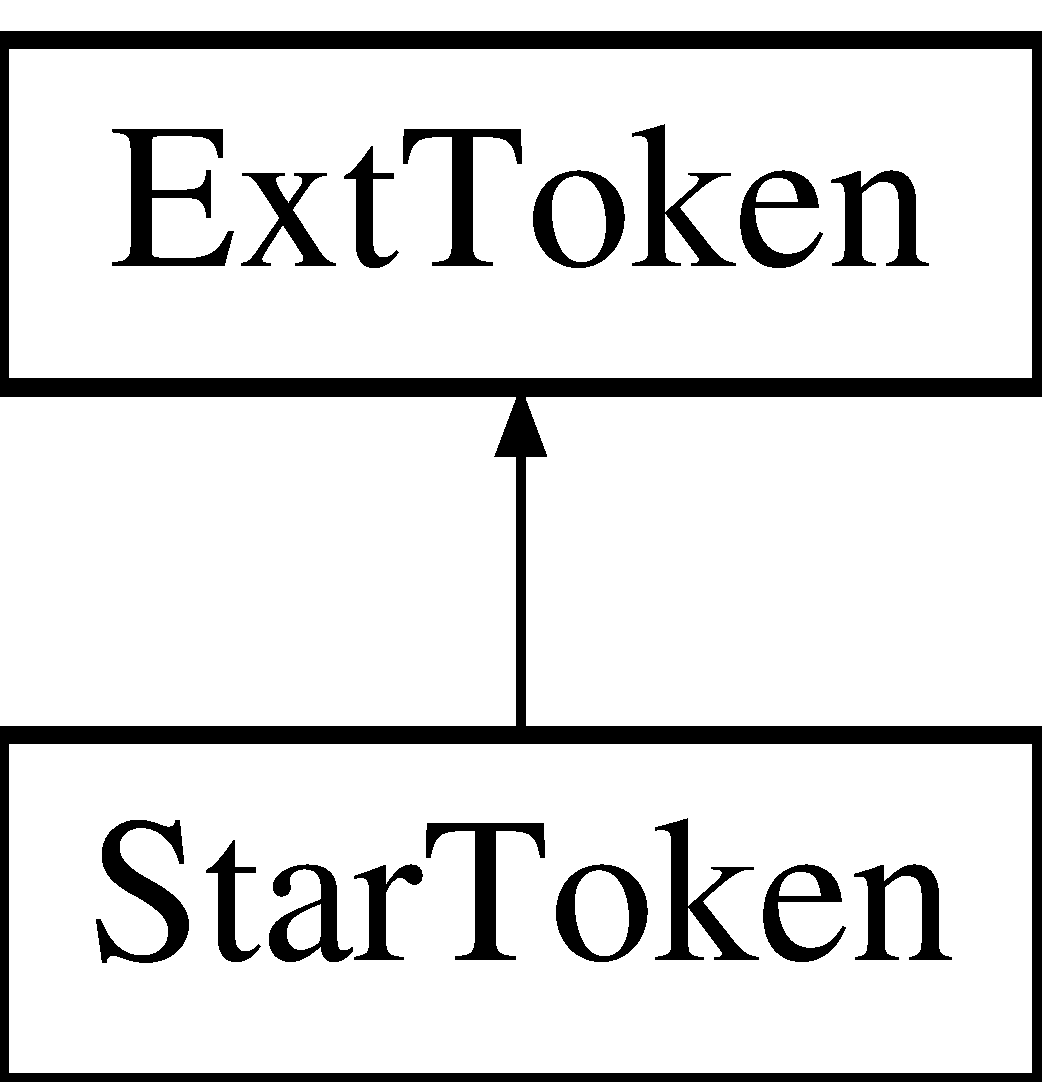
\includegraphics[height=2.000000cm]{classStarToken}
\end{center}
\end{figure}
\subsection*{Public Member Functions}
\begin{DoxyCompactItemize}
\item 
\hypertarget{classStarToken_a9e448a924eb2adbfde602c0590268afd}{{\bfseries Star\-Token} (\hyperlink{classParser}{Parser} $\ast$p, \hyperlink{classToken}{Token} $\ast$t)}\label{classStarToken_a9e448a924eb2adbfde602c0590268afd}

\item 
\hypertarget{classStarToken_aba82bdc81500a58096bfeedad600ad10}{\hyperlink{classParseResult}{Parse\-Result} {\bfseries led} (\hyperlink{classParseResult}{Parse\-Result} left)}\label{classStarToken_aba82bdc81500a58096bfeedad600ad10}

\item 
\hypertarget{classStarToken_a59b81cb08057d75eca4b9a8aad8e2be1}{std\-::string {\bfseries description} ()}\label{classStarToken_a59b81cb08057d75eca4b9a8aad8e2be1}

\item 
\hypertarget{classStarToken_a87682a46d434781795d060e43e7eae23}{int {\bfseries lbp} ()}\label{classStarToken_a87682a46d434781795d060e43e7eae23}

\end{DoxyCompactItemize}
\subsection*{Additional Inherited Members}


The documentation for this class was generated from the following file\-:\begin{DoxyCompactItemize}
\item 
ext\-Token.\-h\end{DoxyCompactItemize}

\hypertarget{classStmt}{\section{Stmt Class Reference}
\label{classStmt}\index{Stmt@{Stmt}}
}
Inheritance diagram for Stmt\-:\begin{figure}[H]
\begin{center}
\leavevmode
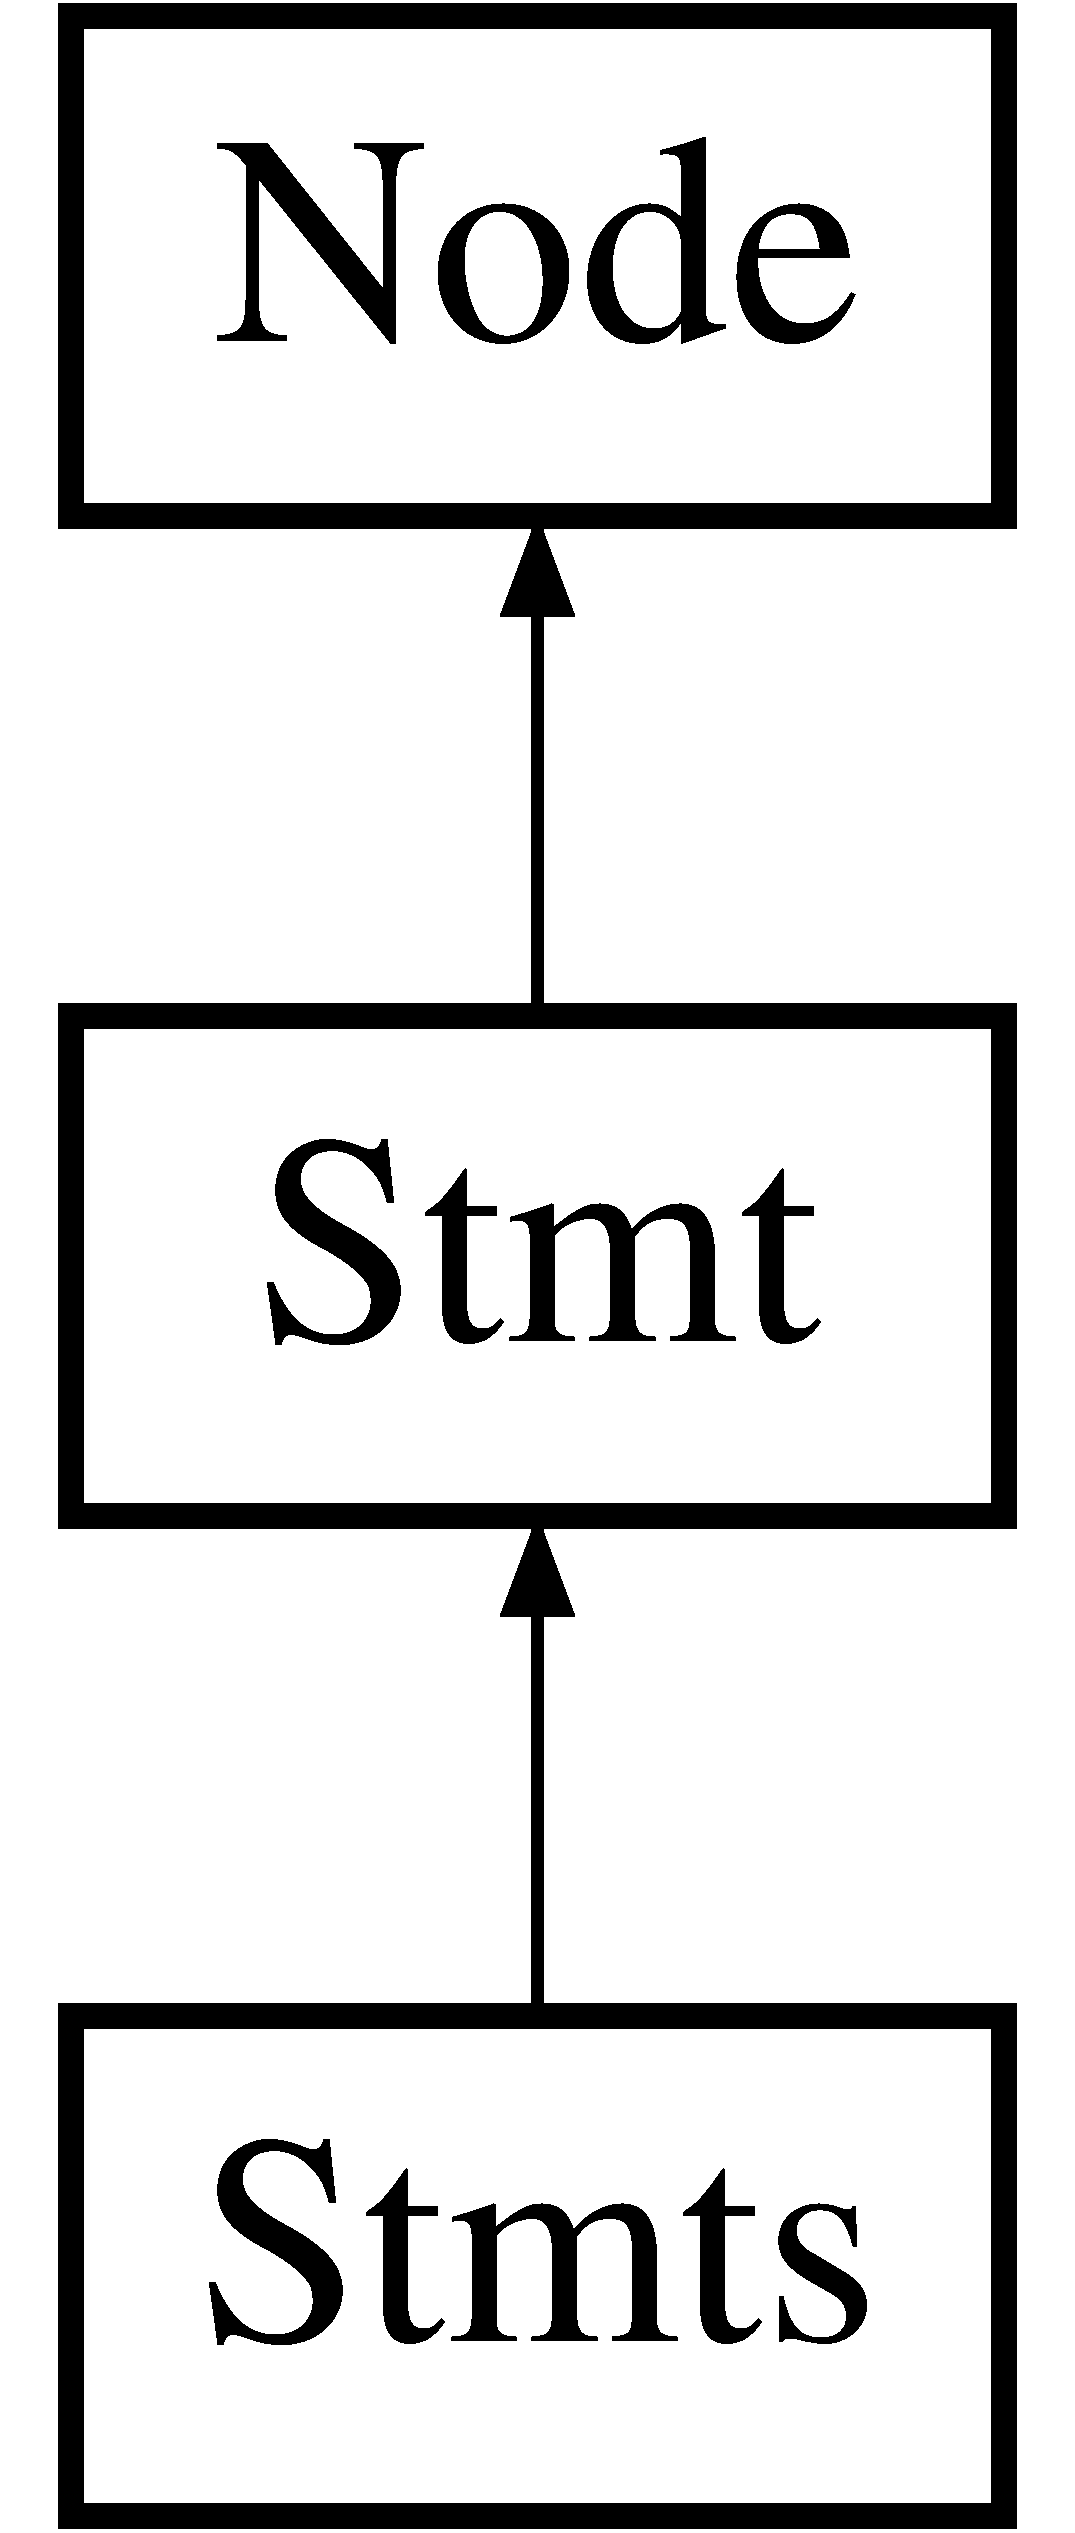
\includegraphics[height=3.000000cm]{classStmt}
\end{center}
\end{figure}
\subsection*{Additional Inherited Members}


The documentation for this class was generated from the following file\-:\begin{DoxyCompactItemize}
\item 
A\-S\-T.\-h\end{DoxyCompactItemize}

\hypertarget{classStmts}{\section{Stmts Class Reference}
\label{classStmts}\index{Stmts@{Stmts}}
}
Inheritance diagram for Stmts\-:\begin{figure}[H]
\begin{center}
\leavevmode
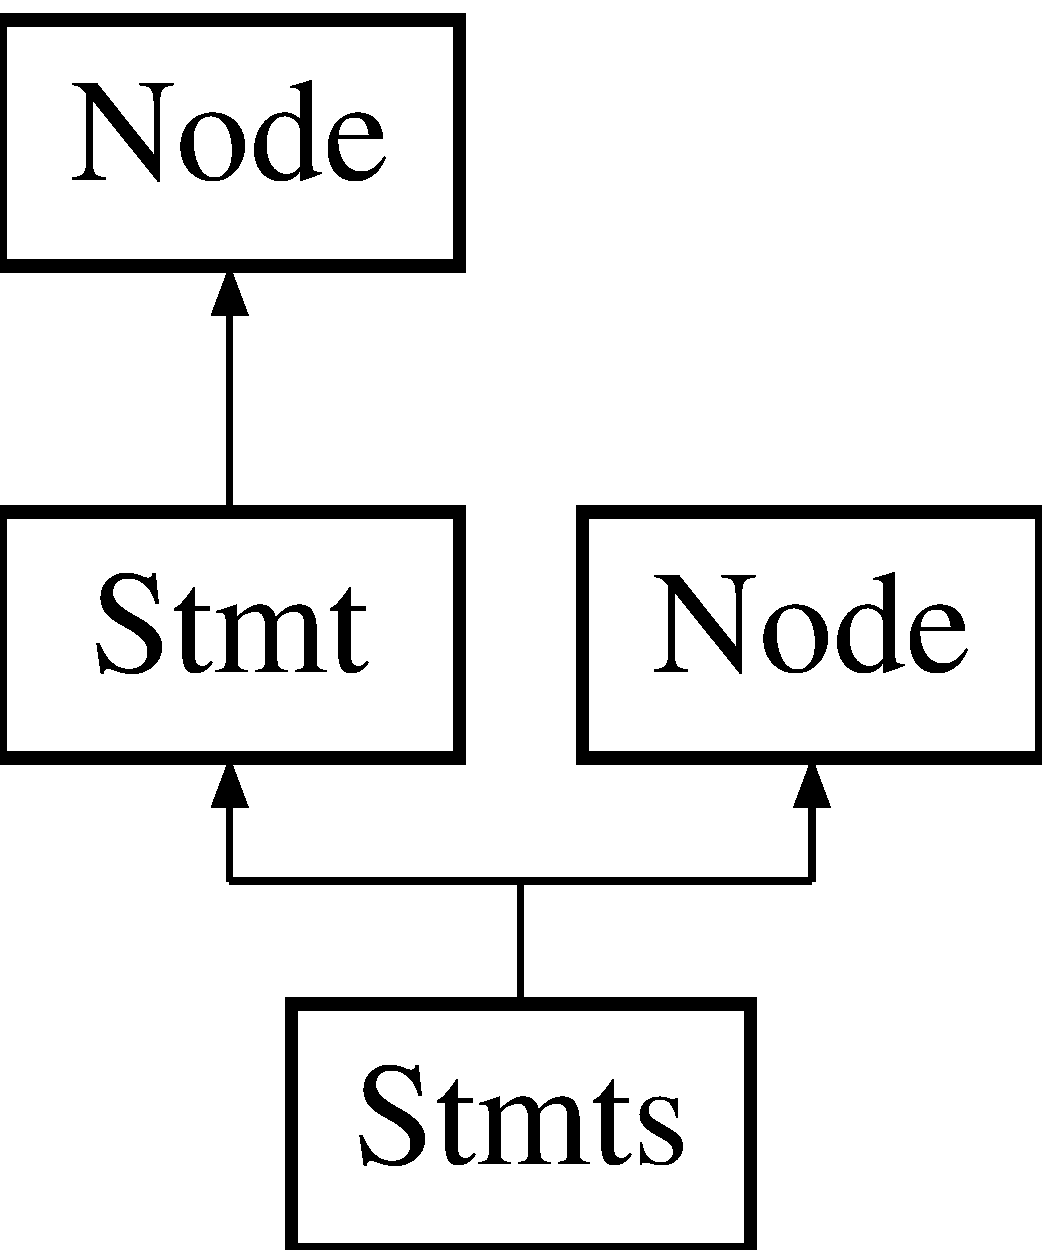
\includegraphics[height=3.000000cm]{classStmts}
\end{center}
\end{figure}
\subsection*{Additional Inherited Members}


The documentation for this class was generated from the following file\-:\begin{DoxyCompactItemize}
\item 
A\-S\-T.\-h\end{DoxyCompactItemize}

\hypertarget{classStringConstToken}{\section{String\-Const\-Token Class Reference}
\label{classStringConstToken}\index{String\-Const\-Token@{String\-Const\-Token}}
}
Inheritance diagram for String\-Const\-Token\-:\begin{figure}[H]
\begin{center}
\leavevmode
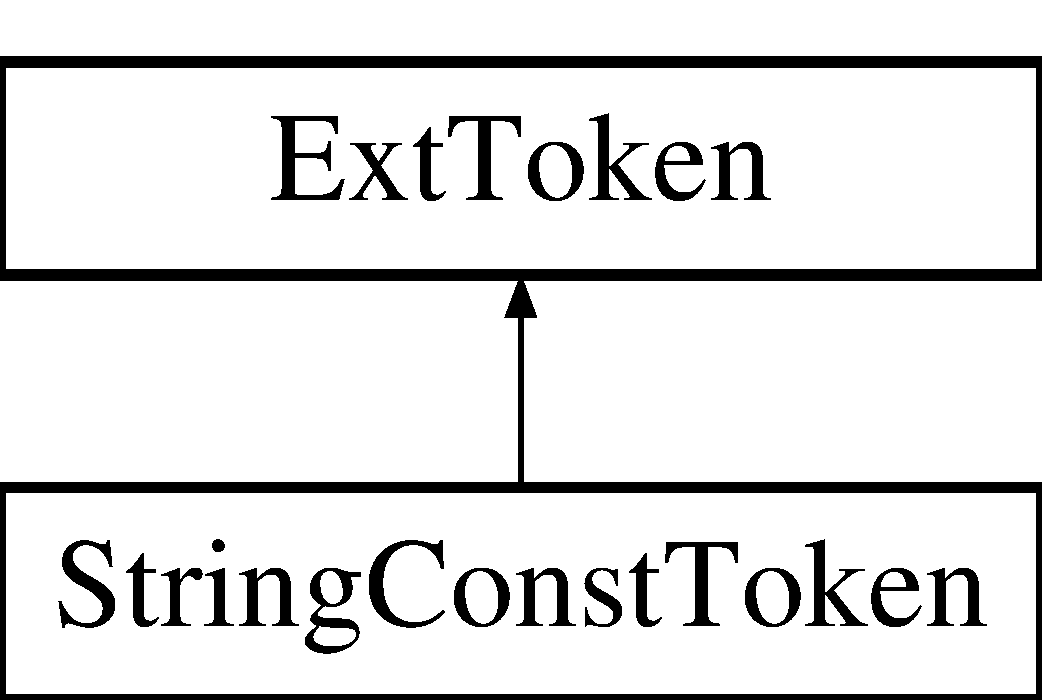
\includegraphics[height=2.000000cm]{classStringConstToken}
\end{center}
\end{figure}
\subsection*{Public Member Functions}
\begin{DoxyCompactItemize}
\item 
\hypertarget{classStringConstToken_aba75cdaef187138a572ba49a5c279fcf}{{\bfseries String\-Const\-Token} (\hyperlink{classParser}{Parser} $\ast$p, \hyperlink{classToken}{Token} $\ast$t)}\label{classStringConstToken_aba75cdaef187138a572ba49a5c279fcf}

\item 
\hypertarget{classStringConstToken_a4767bba84d30289ab31d501f240b80fb}{\hyperlink{classParseResult}{Parse\-Result} {\bfseries nud} ()}\label{classStringConstToken_a4767bba84d30289ab31d501f240b80fb}

\item 
\hypertarget{classStringConstToken_a6343169471a6cb6e422496f2f640691f}{std\-::string {\bfseries description} ()}\label{classStringConstToken_a6343169471a6cb6e422496f2f640691f}

\end{DoxyCompactItemize}
\subsection*{Additional Inherited Members}


The documentation for this class was generated from the following file\-:\begin{DoxyCompactItemize}
\item 
ext\-Token.\-h\end{DoxyCompactItemize}

\hypertarget{classstringDecl}{\section{string\-Decl Class Reference}
\label{classstringDecl}\index{string\-Decl@{string\-Decl}}
}
Inheritance diagram for string\-Decl\-:\begin{figure}[H]
\begin{center}
\leavevmode
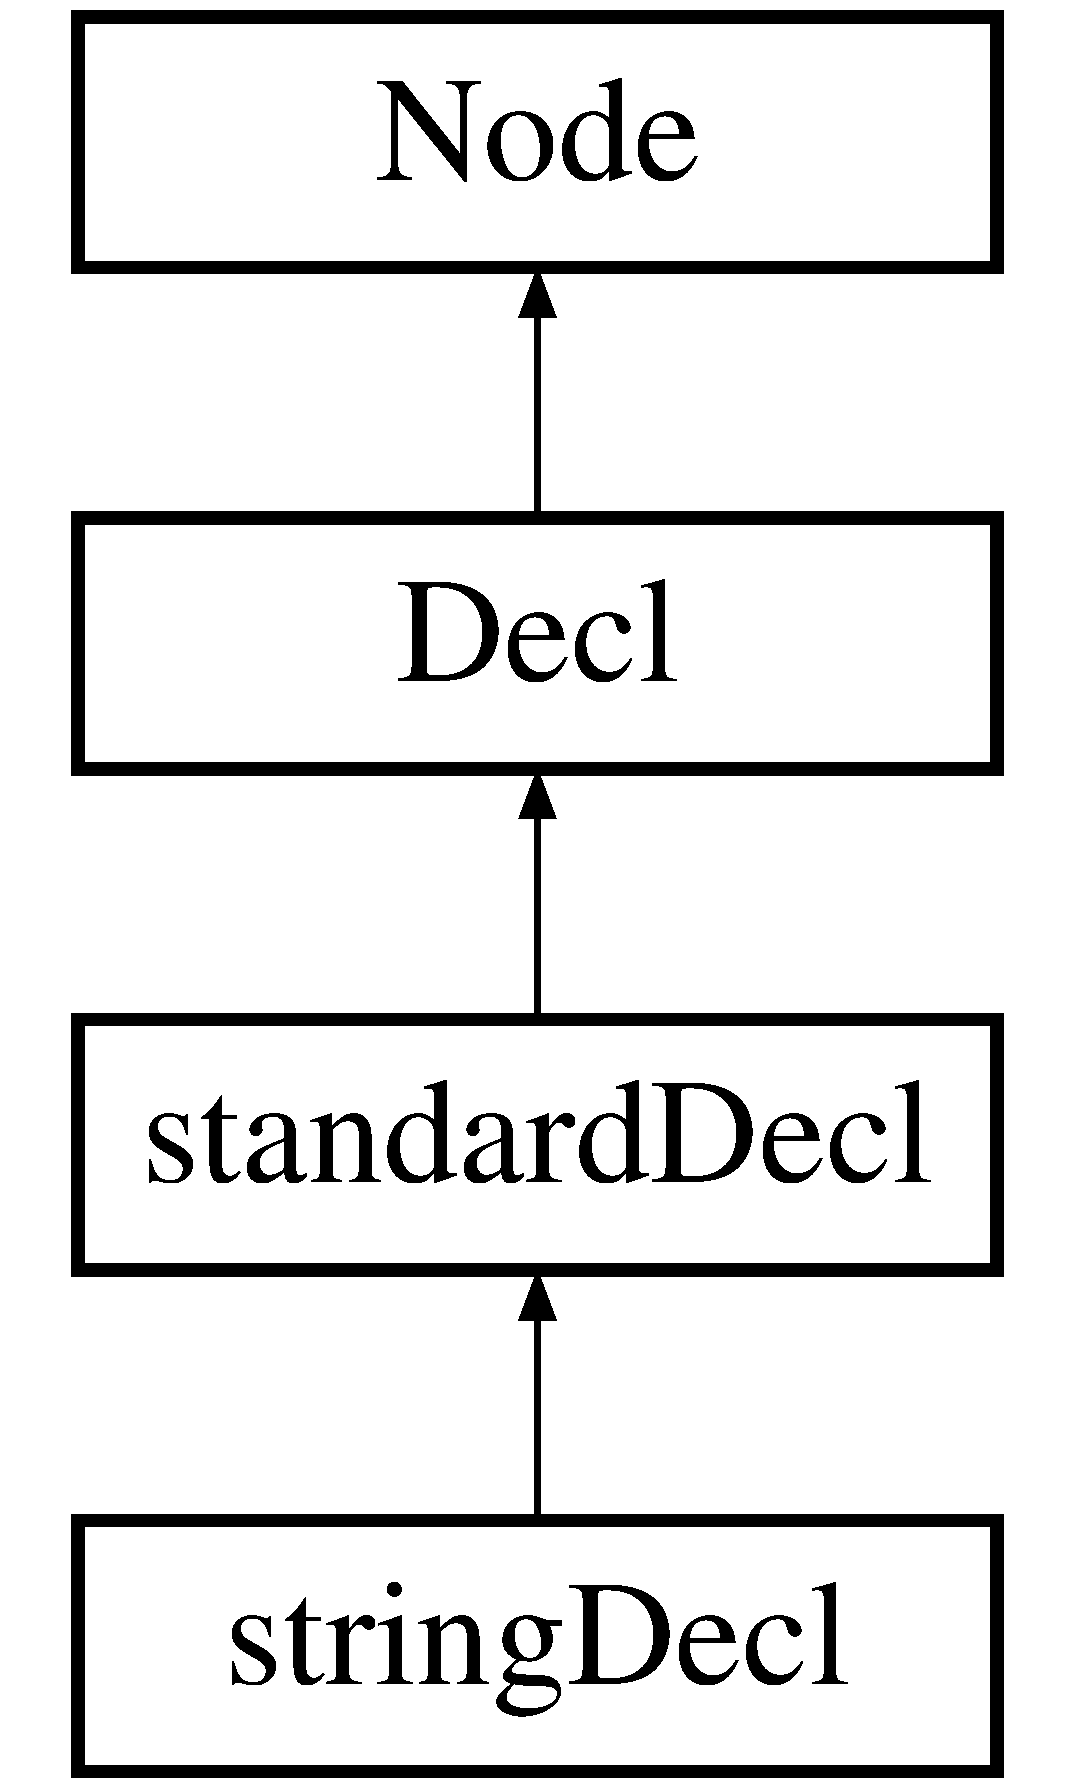
\includegraphics[height=4.000000cm]{classstringDecl}
\end{center}
\end{figure}
\subsection*{Additional Inherited Members}


The documentation for this class was generated from the following file\-:\begin{DoxyCompactItemize}
\item 
A\-S\-T.\-h\end{DoxyCompactItemize}

\hypertarget{classToken}{\section{Token Class Reference}
\label{classToken}\index{Token@{Token}}
}
\subsection*{Public Member Functions}
\begin{DoxyCompactItemize}
\item 
\hypertarget{classToken_a859ef422b90e985ace9f7b4d6cba3e15}{{\bfseries Token} (std\-::string input, token\-Type type, \hyperlink{classToken}{Token} $\ast$next\-\_\-t)}\label{classToken_a859ef422b90e985ace9f7b4d6cba3e15}

\item 
\hypertarget{classToken_a2b1dd7856dd3608aa900015b4951127d}{{\bfseries Token} (std\-::string, token\-Type)}\label{classToken_a2b1dd7856dd3608aa900015b4951127d}

\end{DoxyCompactItemize}
\subsection*{Public Attributes}
\begin{DoxyCompactItemize}
\item 
\hypertarget{classToken_abbff29ede445ed4a8520580f12490832}{std\-::string {\bfseries lexeme}}\label{classToken_abbff29ede445ed4a8520580f12490832}

\item 
\hypertarget{classToken_a11b4722b5e4023d234d2017126de378b}{token\-Type {\bfseries terminal}}\label{classToken_a11b4722b5e4023d234d2017126de378b}

\item 
\hypertarget{classToken_a32f24a25af788c192e5b387dc8d67914}{\hyperlink{classToken}{Token} $\ast$ {\bfseries next}}\label{classToken_a32f24a25af788c192e5b387dc8d67914}

\item 
\hypertarget{classToken_a72a325300d284ac965460fb3a20d9567}{int {\bfseries lex\-Len}}\label{classToken_a72a325300d284ac965460fb3a20d9567}

\end{DoxyCompactItemize}


The documentation for this class was generated from the following files\-:\begin{DoxyCompactItemize}
\item 
scanner.\-h\item 
scanner.\-cpp\end{DoxyCompactItemize}

\hypertarget{classTrueKwdToken}{\section{True\-Kwd\-Token Class Reference}
\label{classTrueKwdToken}\index{True\-Kwd\-Token@{True\-Kwd\-Token}}
}
Inheritance diagram for True\-Kwd\-Token\-:\begin{figure}[H]
\begin{center}
\leavevmode
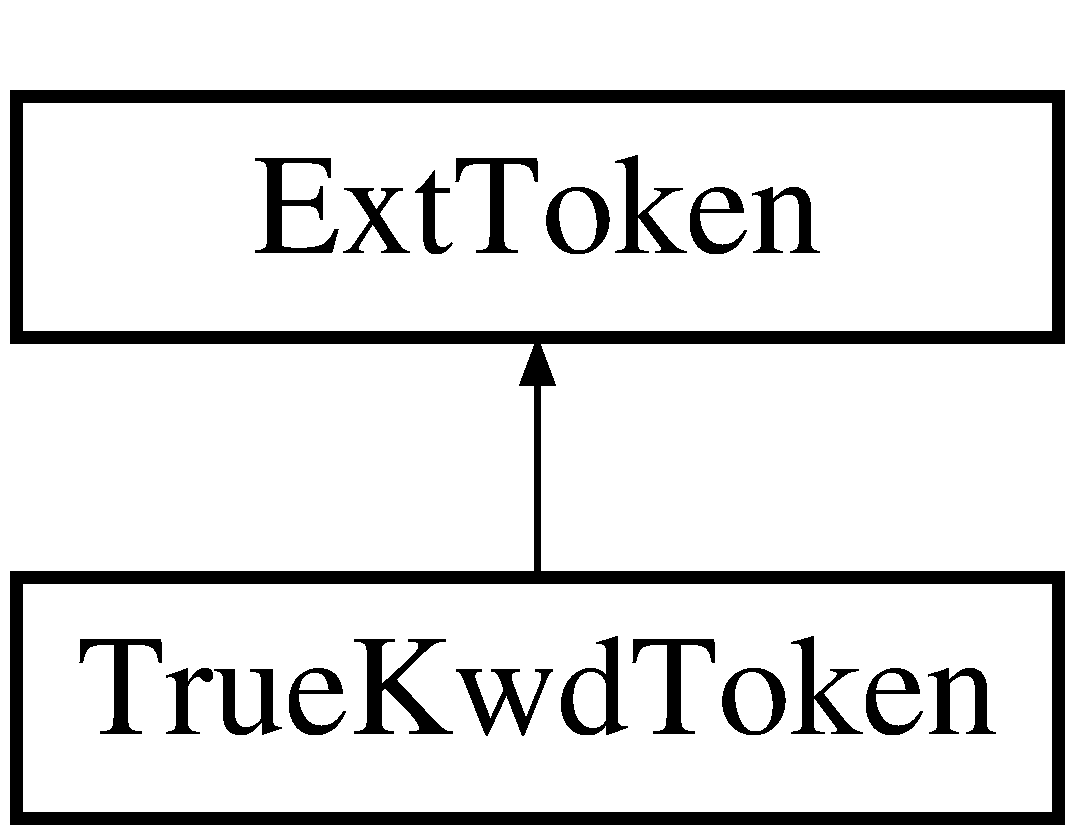
\includegraphics[height=2.000000cm]{classTrueKwdToken}
\end{center}
\end{figure}
\subsection*{Public Member Functions}
\begin{DoxyCompactItemize}
\item 
\hypertarget{classTrueKwdToken_aec070f83a6b91ed35a41e24dfd301b17}{{\bfseries True\-Kwd\-Token} (\hyperlink{classParser}{Parser} $\ast$p, \hyperlink{classToken}{Token} $\ast$t)}\label{classTrueKwdToken_aec070f83a6b91ed35a41e24dfd301b17}

\item 
\hypertarget{classTrueKwdToken_ad86f05acb9483438db153eab44aa6dac}{\hyperlink{classParseResult}{Parse\-Result} {\bfseries nud} ()}\label{classTrueKwdToken_ad86f05acb9483438db153eab44aa6dac}

\item 
\hypertarget{classTrueKwdToken_af4dbe740f06e6928a436d06349af67a9}{std\-::string {\bfseries description} ()}\label{classTrueKwdToken_af4dbe740f06e6928a436d06349af67a9}

\end{DoxyCompactItemize}
\subsection*{Additional Inherited Members}


The documentation for this class was generated from the following file\-:\begin{DoxyCompactItemize}
\item 
ext\-Token.\-h\end{DoxyCompactItemize}

\hypertarget{classVariableNameToken}{\section{Variable\-Name\-Token Class Reference}
\label{classVariableNameToken}\index{Variable\-Name\-Token@{Variable\-Name\-Token}}
}
Inheritance diagram for Variable\-Name\-Token\-:\begin{figure}[H]
\begin{center}
\leavevmode
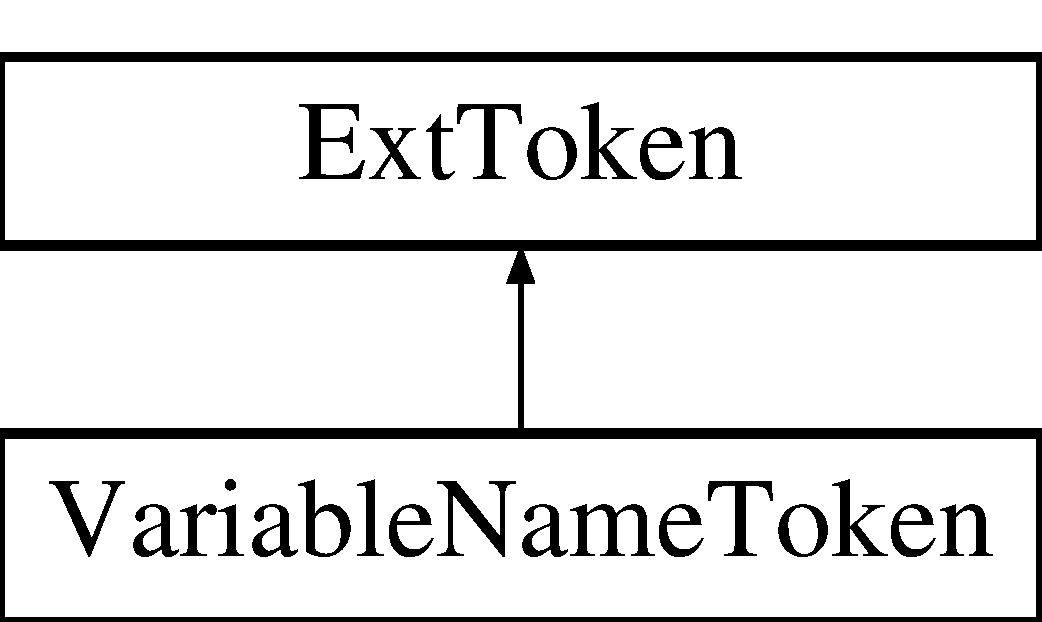
\includegraphics[height=2.000000cm]{classVariableNameToken}
\end{center}
\end{figure}
\subsection*{Public Member Functions}
\begin{DoxyCompactItemize}
\item 
\hypertarget{classVariableNameToken_a804403db425122d1c8d40fd2c6172439}{{\bfseries Variable\-Name\-Token} (\hyperlink{classParser}{Parser} $\ast$p, \hyperlink{classToken}{Token} $\ast$t)}\label{classVariableNameToken_a804403db425122d1c8d40fd2c6172439}

\item 
\hypertarget{classVariableNameToken_a6e775ad5b8c2eafd2e2a185ab90b1f27}{\hyperlink{classParseResult}{Parse\-Result} {\bfseries nud} ()}\label{classVariableNameToken_a6e775ad5b8c2eafd2e2a185ab90b1f27}

\item 
\hypertarget{classVariableNameToken_a54bc3a78736e5c967dc4b1c58e66135b}{std\-::string {\bfseries description} ()}\label{classVariableNameToken_a54bc3a78736e5c967dc4b1c58e66135b}

\end{DoxyCompactItemize}
\subsection*{Additional Inherited Members}


The documentation for this class was generated from the following file\-:\begin{DoxyCompactItemize}
\item 
ext\-Token.\-h\end{DoxyCompactItemize}

%--- End generated contents ---

% Index
\newpage
\phantomsection
\addcontentsline{toc}{chapter}{Index}
\printindex

\end{document}
